\chapter{Phylogenetic lexical flow inference}\label{sec:6}
In many respects, this chapter represents the core of this book. It discusses both the idea of and the methodological difficulties in applying causal inference to data in the shape of overlapping cognate sets in detail, before defining PLFI (phylogenetic lexical flow inference), the first of two algorithms I describe in this book, and then evaluating it on both NorthEuraLex and the simulated scenarios.

This algorithm requires adding reconstructions of all known proto-languages to the model, which makes it causally sufficient, allowing me to work with the much simpler PC algorithm, and postponing the need to get into the complexities of the RFCI algorithm to the next chapter.

In \sectref{sec:6.1}, I discuss possible ways of modeling lexicostatistical data as statistical or information-theoretic variables, and motivate my decision to stick to coarse-grained cognate overlap judgments for the purposes of this book. \sectref{sec:6.2} then introduces my cognate-based information measure, which allows me to derive a very natural measure of conditional mutual information between languages in \sectref{sec:6.3}.

Sections \ref{sec:6.4} and \ref{sec:6.5} are concerned with ways to specialize parts of the PC algorithm in order to balance out assumptions that are not met by conditional independence tests based on this measure. These include the development of an explicitly flow-based criterion for defining plausible separating sets, and of two heuristic criteria for aggregating evidence of directionality. These criteria become necessary because the separating set membership criterion of the PC algorithm is found to be too unstable on cognacy overlap data.

\sectref{sec:6.6} describes how I arrived at the guide tree for my experiments on North\-Eu\-ra\-Lex, which is then used in \sectref{sec:6.7} to perform ancestral state reconstruction in order to create the data for the proto-languages. Before deciding on maximum-likelihood construction as the basis of the PLFI algorithm, I evaluate several alternatives on the simulated data from \chapref{sec:5}.

\sectref{sec:6.8} then puts the results of the previous sections together to define the PLFI algorithm, which is finally evaluated in the last section of this chapter, both on the NorthEuraLex gold standard developed in \chapref{sec:4}, and the simulated data from \chapref{sec:5}.

\section{Modeling languages as variables}\label{sec:6.1}
Everything starts with the idea of detecting conditional independence relationships between sets of languages, making it possible to apply causal inference algorithms to the lexical flow inference task. To take up the idea foreshadowed by the language examples in \chapref{sec:3}, I will assume the lexicon of each language to quite literally be caused by the lexicon of its ancestor language and possibly other languages which influenced its development. Put differently, the model is intended to determine how the lexicon of a language came about as a mixture of lexical material from other languages, and summarize the results in a causal graph.

As the crucial step towards this goal, we need a formalism which makes it possible to treat languages as information-theoretic variables. Depending on a range of choices about how we model languages, there are many possibilites to define useful measures of information content and mutual information between languages. While a single rather simple measure on cognate sets will be used later, in this section the idea will be put into a wider context by discussing more generally the different ways in which languages might be treated as statistical or information-theoretic variables.

\subsection{Languages as phoneme sequence generators}\label{sec:6.1.1}
The reductionist premise of lexicostatistical databases is to view each language simply as a (possibly many-to-many) mapping from concepts to lexical realizations. This means we could treat languages as variables generating sequences of phoneme n-grams, and measure information-theoretically how much about the generated sequence in one language we know given the sequence generated by another language. For unrelated languages, we could expect the mutual information to be not significantly different from zero. A significance threshold for an independence test could be based on the amount of mutual information we would expect if the two word lists were randomly sampled from the two languages.

The question what a good sampling procedure would look like, is quite involved, and again depends on how we model the generated phoneme sequences. The most straightforward way to model the phoneme emission would be to use n-gram distributions, to treat concept realizations as events producing bags of n-grams, and measure the mutual information between the resulting distributions. This is a formal answer to the intuitive question: given the n-grams for a realization of some concept in language A, how much on average do we already know about the realization of the same concept in language B? To come back to one of our examples from \chapref{sec:3}, the phonetic bigram representations of \textit{slange} [slɑŋə] and \textit{Schlange} [ʃlɑŋə], the \ili{Danish} and \ili{German} words for `snake', share three out of four elements (\{[lɑ], [ɑŋ], [ŋə]\}, giving them a very high mutual information, whereas knowing either word does not help us at all to predict the \ili{Finnish} equivalent \textit{käärme} [kæærmɛ], which does not share a single bigram with the Germanic words.

While this is an attractive idea, initial exploratory experiments quickly show that the information content of n-gram overlaps is not very high. For instance, the global bias towards CVCV-type syllable structures will lead to spurious mutual information, as e.g.\ CV-type bigrams such as [pa] or [ku] will always be more common than CC or VV-type n-grams.

The realization-based mutual information measure can be somewhat improved upon by building it only on aligned positions. Essentially, we optimally align all the realizations for each pair of languages, count how often each pair of n-grams (for reasons of data sparseness, only unigrams and bigrams are feasible) is aligned, and compare this to the distribution we would expect if the words were randomly chosen. Again, the threshold needs to be computed by resampling, because the two n-gram distributions computed in this way will not be independent due to the fact that the alignment algorithm will always find some vowels (and often some consonants) to align even in completely random and unrelated words. In exploratory experiments, the necessary threshold turned out to be so high that the common signal between languages from different branches of Indo-European could not be distinguished from noise. While it might be possible to arrive at a sufficiently sensitive independence test by refining this approach, the process is hampered by the fact that error causes are very difficult to track down and interpret in such a model.

\subsection{Languages as cognate set selectors}
A third possibility (and the one which I am going to build upon) starts with structures that are situated one step higher in the usual toolchain of computational historical linguistics. Assume we have a good cognate detection method in place. Then, we can use this module to group the realizations of each concept $i$ into a set of cognate sets $Cog_i := \{cog_{i,1}, \dots, cog_{i,n_{i}}\}$.

In terms of a probabilistic model, this leaves us with a quite complex chain of random variables building on the basic view of languages as string generators. For each language $j$, we could start with a lexicon generator variable $Lex_j \colon \Omega \rightarrow \Sigma^*$ for some universal alphabet $\Sigma$ of phonetic symbols. Possible observations of such a variable could be phonetic strings such as [æææ], [ktkəəŋ], and infinitely many other highly improbable strings. Alternatively (and especially to model resampling), $Lex_j$ can be defined as selecting strings from a predefined set $L_j \in \Sigma^*$ containing all the strings of the lexicon, that is, in our case, a phonetic representation of all the lemmas in our database. On the NorthEuraLex data, the English variable would generate words such as [taʊn], [fiːvə], [hɛvɪ], [aɪ], but the assignment of these forms to meanings would be assumed to be entirely random.

Any automated cognate detection procedure can now be conceptualized as a very complex function of all the lexicon generator variables which generates a set of cognate sets for each concept $C_i$:
\begin{equation*}
 cog(X_1,\dots,X_n)\ \colon\ \Omega \rightarrow \bigotimes_{i = 1}^{n} \wp\left(\bigcup_{j=1}^{m} Lex_j\right)^*
\end{equation*}
Unrelated languages can now be seen as independently sampling one or several of these cognate sets for each given concept. For related languages, we should then be able to measure a dependence in the form of non-zero mutual information. Intuitively, the more closely two languages are related, the more knowing which cognate sets one language picked will help us to predict the sets picked by the other language. If we know for one Germanic language (such as German) that it picked its word for `honey' from the cognate set of English \textit{honey}, this will be much more helpful for predicting to which class the \ili{Icelandic} word will belong, than knowing the cognate set of the equivalent in a more distantly related language like \ili{Greek}.

Mathematically, we can now model each language $L_j$ as a variable picking for each concept a random subset of the set of cognate sets, i.e.:
\begin{equation*}
  L_j: \Omega \rightarrow \bigotimes_{i = 1}^{n} \wp(Cog_i)
\end{equation*}
From a probabilistic point of view, this is the shape of the variables I am going to operate on, although it would be very difficult to assign explicit joint probability distributions to sets of such variables. Instead, I will only use an information geometry on these variables.

\section{A cognate-based information measure}\label{sec:6.2}
We now turn to the question of how to estimate conditional mutual information between languages modeled as cognate set selectors. The basic idea is to define an easy-to-compute and intuitive measure $h$ on outcomes of cognate set selection, which mimics joint entropy in adhering to the basic properties of a submodular information measure. Based on this measure, I will then be able to define an equivalent of conditional mutual information between languages.

A simple information content measure $i$ turns out to be easy to find: one can simply define $i(L_j)$ for a language variable $L_j$ as the number of cognate sets selected by the language across concepts:
\begin{equation*}
 i(L_j) := \sum_{i = 1}^n | L_{j,i}(\omega)|
\end{equation*}
I will treat this definition as the self-information of $L_j$, i.e.\ the outcome of a random variable measuring the entropy of language $L_j$. There is a very intuitive parallel between this measure and the view of entropy as a measure of descriptive complexity: given a set of concepts and a set of cognate sets for each concept, the minimum description length for the lexicon of $L_j$ can be seen as the length of the minimal specification of the mapping from concepts to cognate sets, which will be linear in the number of cognate sets touched by the language.

The equivalent of the joint entropy $h(L_j,L_k)$ can now be defined as the number of cognate sets selected by one of the two languages, i.e.\ the union of the outcomes represented by both languages: 
\begin{equation*}
 h(L_j,L_k) := \sum_{i = 1}^n | L_{j,i}(\omega) \cup L_{k,i}(\omega)|
\end{equation*}
Analogously, we can define $h(\mathbf{Z})$ for all subsets $\mathbf{Z} = \{Z_1,\dots,Z_m\} \subseteq \mathcal{L}$ of our set of languages $\mathcal{L}$. In Appendix C, I show that this measure adheres to the elemental inequalities defining a submodular information measure. According to the theory introduced in \sectref{sec:3.2.2.3}, this establishes that the measure $h(\mathbf{Z})$ for a set of languages $\mathbf{Z} = \{Z_1,\dots,Z_m\}$, is similar enough to a measure of joint information to lead to a consistent definition of conditional mutual information.

We have seen previously how cognacy data can be pictured as representing each language as a long binary vector in which each dimension represents a cognate set, and the values 1 and 0 represent the presence or absence of each cognate set in that language. By the information measure just introduced, the information content $i(L_j)$ of a language $L_j$ is then simply the number of ones in its vector representation, and the joint entropy is the number of ones in the disjunction of the language vectors, i.e. the vector which has a zero in the components where every language vector has a zero, and a one in all components where at least one language vector has a one. This representation is of course very sparse, since there will sometimes be dozens of cognate classes for any given concept observed across a hundred languages. Measures based on such a representation can be expected to be very prone to sampling errors, e.g. if a cognate for a word exists in a language, but simply was not attested in our lexical 
resource, or it has shifted slightly in meaning, which is why we do not observe the full path. 

Structurally, these problems are very similar to the reasons why the idea of learning more dense embeddings of such sparse vectors in a lower-dimensional space has gained a lot of traction in computational linguistics, leading to a variety of techniques for distributed representations which are summarized e.g. by \cite{goldberg2016}. The general idea of applying embeddings here would be to find a good representation of the cognacy features for each concept as vectors in a lower-dimensional vector space, so that concepts which pattern similarly across languages will have similar representations. The representations of the cognate sets picked by a language would then be concatenated to form a more dense language vector. This procedure allows information sharing between cognate set presence or absence features, which would not only correct for the fact that the features are not independent (because generally, already having a word from cognate class A for some concept makes it less likely that it will also have a word from cognate class B for it), but also provide a way of smoothing out gaps in the data based on the knowledge provided by similar languages (e.g. predicting that the word for `honey' in any Germanic language will belong to the same cognate class as English \textit{honey}, even if for some reason there is a gap in the database).

On such embedded cognacy vectors, conditional independence tests could be defined e.g. through cosine similarities or Pearson correlations (after centering), but it would also very likely be possible to define a joint entropy measure $h(L_j,L_k)$ based on combinations of embedding-based language vectors. While given the experience in mainstream areas of natural language processing, such representations would very likely yield better results due to better information sharing, its results would no longer be interpretable in terms of discrete lexical transmission events, and the resulting notion of lexical flow would only be a very abstract information-theoretic measure instead of being directly mappable to the paths by which certain words traveled. In this book, I will therefore only explore the count-based joint entropy measure defined above, and leave the exploration of embedding-based measures to future work.

\section{Conditional mutual information between languages}\label{sec:6.3}
To arrive at the needed measure of conditional mutual information $i(L_i;L_j|\mathbf{Z})$, I can now simply use the standard definition on the information measure: 
\begin{equation*}
 i(L_i;L_j|\mathbf{Z}) = h(L_i,\mathbf{Z}) + h(L_j,\mathbf{Z}) - h(L_i,L_j,\mathbf{Z}) - h(\mathbf{Z})
\end{equation*}
Applying the definition of $h$ I just developed, and writing $cog(L_1,...,L_k)$ for the set of cognate sets shared by the languages $L_1,\dots,L_k$, $i$ becomes a count of conditional cognate overlap, which can be seen intuitively as the number of items in unblocked lexical flow. Note that the blocking of information flow was also the intuition behind the concept of d-separation which I introduced in \sectref{sec:3.1.2.1}, and the close correspondence between conditional independence constraints and d-separation in Bayesian networks is what will make it possible to infer networks via sequences of tests for vanishing conditional cognate overlap.

In order to be able to define a global threshold value for conditional independence tests, conditional mutual information needs to be normalized by the number of remaining cognates not touched by any of the conditioning languages, yielding the normalized conditional mutual information $I(L_i;L_j|\mathbf{Z})$:

\begin{equation*}
 I(L_i;L_j|\mathbf{Z}) := \frac{|cog(L_i,L_j)\backslash\{c\ |\ \exists \{Z_1,\dots,Z_k\} \subseteq \mathbf{Z}\colon c \in cog(Z_1,\dots,Z_k)\}|}{\max\{|cog(L_i,Z_1,\dots,Z_k)|,|cog(L_j,Z_1,\dots,Z_k)|\}-|cog(Z_1,\dots,Z_k)|} 
\end{equation*}

Informally, $I(L_1;L_2|Z)$ thus quantifies the share of cognates between $L_1$ and $L_2$ which cannot be explained away by having been borrowed through a subset of the languages in $Z$. To use this measure of dependence as a conditional independence test, we simply check whether $I(L_1;L_2|Z) \leq \theta_{L_1,L_2}$ for a threshold $\theta_{L_1,L_2}$, which could be derived from the number of false cognates between $L_1$ and $L_2$ which we expect due to automated cognate detection. In practice, I am setting $\theta_{L_1,L_2} := 0.025$ for all language pairs because the distribution of false cognates is difficult to estimate, and language-specific thresholds did not lead to better results in initial experiments on a smaller language set. On the NorthEuraLex data, this means that languages which share 25 cognates or less will be unconditionally independent, and every link the algorithm establishes will explain an overlap of at least 26 cognates.

Based on this conditional independence test, the first stage of the PC algorithm will derive a causal skeleton which represents a scenario of contacts between pairs of input languages that is only as complex as necessary to explain the lexical overlaps. The model thus assumes that all similarities are primarily due to mutual influence, and never infers the existence of hidden common causes, such as proto-languages. As we shall see, to arrive at a phylogenetic network, we will need to introduce the proto-languages as additional variables.

\section{Improving skeleton inference}\label{sec:6.4}
When applying my newly developed conditional independence test to small test cases, it quickly becomes clear that they do not reflect the constraints defined by the gold standards very well. The main problem for skeleton inference is the way in which separating set candidates are selected in the PC and PC* algorithms. In this section, I develop an alternative to these two standard candidate selection techniques, and a comparison of the performance of all three variants will be part of the evaluation at the end of this chapter.

\subsection{Problem: stability on discrete information}
The PC algorithm as presented in \sectref{sec:3.2.3} is only tractable because it tests separating set candidates by ascending order of cardinality, and builds on the assumption that any separating set must be a subset of immediate neighbours of $L_i$ and $L_j$ in the current skeleton. Conditioning on any set of neighbours is possible in the vanilla PC algorithm because the faithfulness assumption implies that true dependencies will always ``shine through'', no matter how many intervening variables we condition on. For our model, this is a problematic assumption, because being allowed to select any neighbours makes it too easy to screen off languages from each other in our information geometry of limited granularity.

A small simplified example based on the NorthEuraLex data will show why this is a problem for skeleton inference. In the gold standard, there is a contact link between \ili{Norwegian} (\iso{nor}) and \ili{Southern Saami} (\iso{sma}). In the cognacy data, we have $|cog($\iso{nor}$,$\iso{sma}$)| = 114$, i.e.\ the two languages share 114 cognate sets, of which some are false positives, but most reflect North Germanic\il{North Germanic languages} loans. At some stage of skeleton inference, \iso{sma} is still connected to its neighbour \ili{Northern Saami} (\iso{sme}), and one of the remaining neighbours of \iso{nor} is \ili{Swedish} (\iso{swe}). Now, most of the North Germanic material is of course also present in Swedish, leaving a quite high overlap $|cog($\iso{sma}$,$\iso{swe}$)| = 111$, a large part of which is shared between all three languages: $|cog($\iso{nor}$,$\iso{sma}$,$\iso{swe}$)| = 96$. Using these overlaps, we first get a successful conditional independence test (\iso{nor} $\indep$ \iso{sma}\ |\ \iso{swe}), because

\fittable{
\parbox{1.2\textwidth}{
\begin{equation*}
\begin{split}
I(\mathit{nor};\mathit{sma}\ |\ \mathit{swe}) & = \frac{|cog(\mathit{nor}) \cup cog(\mathit{swe})|+|cog(\mathit{sma}) \cup cog(\mathit{swe})|}
     {\max(|cog(\mathit{nor}) \cup cog(\mathit{swe})|,|cog(\mathit{sma}) \cup cog(\mathit{swe})|)-|cog(\mathit{swe})|}\\
     & - \frac{|cog(\mathit{nor}) \cup cog(\mathit{sma}) \cup cog(\mathit{swe})| + |cog(\mathit{swe})|}
     {\max(|cog(\mathit{nor}) \cup cog(\mathit{swe})|,|cog(\mathit{sma}) \cup cog(\mathit{swe})|)-|cog(\mathit{swe})|}\\
     & = \frac{18}{1008} = 0.018
\end{split}
\end{equation*}
}
}

Now, after deleting the link \iso{nor} $\arrowLL$ \iso{sma} due to the successful test, the neighbour relation between Norwegian and Swedish persists, also giving us (\iso{swe} $\indep$ \iso{sma}\ |\ \iso{nor}), so that the resulting skeleton lacks any hint of the contact between North Germanic and Western Saami.

This example demonstrates that for skeleton inference to work on my coarse-grained data, the decision to remove a link between two languages should not be based only on the numbers of cognates shared with some set of immediate neighbours. The PC* algorithm already goes one step towards the solution by considering only neighbours on connecting paths, but this will not solve the problem in this case, either: There is a connecting path \iso{nor} $\arrowLL$ \iso{swe} $\arrowLA$ \iso{fin} $\arrowOA$ \iso{sme} $\arrowLL$ \iso{sma}, which would also make \iso{swe} a possible element for separating set candidates, causing exactly the same problem.

\largerpage
\subsection{Flow Separation (FS) independence}
We will now see how it is possible to at least partially correct for the lack of faithfulness by exploiting the fact that we have more than just a single conditional mutual information value to perform each conditional independence check. $I(L_i;L_j|\mathbf{Z})$ is computed from as many as 1,016 individual ``concept stories'' which provide us with a much richer picture of what is going on, and can help us to quantify the information flow much more precisely. To explain away a cognate that is shared between two languages $L_i$ and $L_j$, it must have been possible for the lexeme in question to have travelled between the two languages on some other path. Therefore, any minimal separating set must form a union of acyclic paths between $L_i$ and $L_j$. In effect, this constitutes an explicit model of the lexical flow helping us to decide more reliably which links can be deleted. In our example case, we now get $I($\iso{nor}$;\ $\iso{sma}$\ |\ \mathcal{L}\backslash\{$\iso{nor}$,$\iso{sma}$\}) = 0.051$, i.e.\ the link will correctly not disappear whichever 
separating set candidate we condition on.

The adapted mutual information measure will be called \textit{\isi{flow separation (FS)}}. Adopting the convention of using two-letter shorthands for the different skeleton inference methods, \textit{PC} will be used for the vanilla PC variant, and \textit{PS} as a shorthand for PC* (``PC-Star''). My implementation of FS uses a depth-first search of the current graph to get all connecting paths which contain four nodes or less, and generates all combinations of these paths which lead to separating set candidates of a given cardinality. Longer paths would need to be considered in theory, but did not lead to different results on my data, at a much higher computational cost. The cognate sets for each concept are tested separately against these paths in a highly optimized fashion, making the FS-based independence test not significantly slower than the PC and PS variants.

\section{Improving directionality inference}\label{sec:6.5}
Similar problems in applying the vanilla PC algorithm face us in directionality inference, the second stage of constraint-based causal inference algorithms. The two standard v-structure detection procedures which were already introduced in \chapref{sec:3}, will from now on be referred to as \textbf{VPC} (\textbf{V}anilla \textbf{PC}) and \textbf{SPC} (\textbf{S}table \textbf{PC}). Both of these variants build on the separating sets used to infer the skeleton, but the uncertain nature of independence checks on our data again forces us to explore alternative approaches. The first variant only replaces v-structure detection and then works with the propagation rules from Stage 3 of the PC algorithm, and the second variant I will introduce here tries to infer the directionality signal independently of the skeleton. In both cases, the basic idea behind directionality detection will still be informed by the theory of causal inference.

\subsection{Problem: monotonic faithfulness and v-structures}
To recapitulate, in the second stage of the PC algorithm and related algorithms, VPC and SPC directionality inference on the causal skeleton is performed by asking whether the central language $B$ in each pattern of the form $A \arrowLL B \arrowLL C$ was part of the separating set that was used for explaining away the link $A \arrowLL C$. The idea is that if $B$ was not necessary to explain away any possible correlation between $A$ and $C$ (i.e.\ there is a separating set not containing $B$), this excludes all causal patterns except $A \rightarrow B \leftarrow C$. This is based on the assumption that in each of the three other possible causal scenarios, we would see some information flow between $A$ and $C$ if we do not condition on $B$.

This type of reasoning is again justified by the causal faithfulness assumption, which states that we can derive exactly the conditional independence relations implied by the true graph through d-separation. More specifically, the scenario $A \rightarrow B \leftarrow C$ would be characterized by the conditional independences $A \indep C$ and $(A \notindep C\ |\ B)$, whereas $(A \indep C\ |\ B)$ would hold in all other scenarios for the unshielded triple $A - B - C$.

Unfortunately, this version of faithfulness only holds in the probabilistic case, and does not apply to information-theoretic causal inference. If we have $A \indep C$, it necessarily follows that $(A \indep C\ |\ B)$, which means that we will never encounter the pattern characterizing $A \rightarrow B \leftarrow C$, because of a spurious independence $(A \indep C\ |\ B)$ that is not induced by d-separation. In our application to languages, the problem can be made intuitive by stating that additional languages can only be used to ``explain away'' cognates for a given language pair, but we will never find additional cognates given the information from other languages.

\cite{steudel_ea_2010} show that the independence relations derived from a submodular information measure still follow a weaker notion of faithfulness, which they call \textit{\isi{monotone faithfulness}}. Monotone faithfulness relaxes the enforced correspondence between d-separation and conditional independences by only requiring that $(A \indep C\ |\ \mathbf{B})$ implies d-separation of $A$ and $C$ by a set $\mathbf{B}$ if $\mathbf{B}$ is minimal among all conditioning sets that render $A$ and $C$ independent. It turns out that the correctness proof for the PC algorithm can be adapted directly to show that it will return monotonically faithful representations if the input consists of monotonically faithful observations.

So what does this mean for the results of the PC algorithm on my cognate data? Even the weaker requirement of monotonic faithfulness still implies the very strong assumption that every scenario in which $A$ has an influence on $B$ and $B$ on $C$, this would become visible as a dependence between $A$ and $C$ (because $A$ and $C$ would not be d-separated by the empty set). While this assumption may be unproblematic for continuous statistical variables, we cannot expect it to hold for my information-theoretic notion of independence. Again, the underlying problem is that I am modeling languages (and mutual information between them) as discrete sets of entities (or their overlap), which is far too coarse-grained to detect clean and consistent causal signals.

The assumptions behind the PC algorithm therefore imply the following statements which do not hold for languages: 
\begin{itemize}
 \item If two unrelated languages borrow from a third language ($A \leftarrow B \rightarrow C$),
 some words will always be borrowed into both languages ($I(A;C) \neq 0$).
 \item If one language influences another one which in turn influences a third one ($A \rightarrow B \rightarrow C$),
 this will always cause some lexical material to be transferred from the first one to the third ($I(A;C) \neq 0$).
\end{itemize}
While the first assumption might be defendable in my model (it is indeed very common that e.g.\ a language with state support leaves some common core of lexical items in all minority languages), the second one is extremely problematic, since it is easily conceivable that if a language $A$ borrows from a language $B$ which in turn borrows from a language $C$, none of the lexical material from $C$ will appear in $A$, especially if there is a temporal order to these contacts.

For our information-theoretic language variables, the inadequacy of the faithfulness assumption leads to many erroneous v-structures and a chaotic picture if we apply the second stage of the PC algorithm as is. In addition, since there will often be many separating sets of the same size, we are quickly faced with a well-known weakness of the PC algorithm: The results of its second stage are highly dependent on the order in which separating set candidates are tried out. In practice, this means that many possible orders have to be tested, often giving rise to conflicting evidence which needs to be reconciled. Crucially, this implies that we cannot directly rely on the separating sets to detect v-structures in a way that is robust enough for propagation as in the PC algorithm. Instead, we need a more robust way of detecting v-structures in cognate overlap patterns.

\subsection{Unique Flow Ratio (UFR): flow-based v-structure testing}
Above all, it is the lack of reliability in the independence tests which will lead to chaotic results if the separating set criterion is applied in the standard way. This lack of reliability is partially caused by erroneous cognacy judgments (which could be improved by hand-crafted annotations), but more importantly by a lack of statistical power in tests which involve distantly related languages, i.e.\ where the lexical overlaps only consist of a handful of items. But, even if the independence tests are correct (and they are more likely to be thanks to the FS criterion), there are typically many alternative separating sets, indicating that not much useful information can be extracted from the fact that a language was contained in some separating set.

To improve on the situation, and develop an alternative v-structure test which gets the maximum out of the little data I have available in my application, I need to get back to the motivation why the PC-algorithm and its variants detect v-structures by considering separating sets in unshielded triples. The essential idea justifying the inference of a v-structure $A \rightarrow B \leftarrow C$ was to decide whether $B$ was necessary to separate $A$ and $C$ by inspecting the separating sets, and seeing whether $B$ was in all (VPC) or the majority (SPC) of them.

Can this basic idea be applied more directly to the cognate set overlaps between languages? It turns out that a flow-based criterion can also help us here, as we can explicitly calculate how much of the overlap between $A$ and $C$ can only be explained via paths involving $B$ on the causal skeleton. The essential idea is thus the same as the one behind the flow-separation independence test.

Let $c(L_1,\dots,L_k) := |cog(L_1,\dots,L_k)|$ be the number of cognate IDs shared between between all the languages $L_1,\dots,L_k$, and define $c(A-B-C)$ (the \textit{\isi{unique flow}}) as the number of cognates which no path excluding $B$ could have transported between $A$ and $C$. Now, we can quantify the answer to the question how much $B$ is needed to remove $A \arrowLL C$ based on the answers of two simpler questions. The first question is whether there is as much unique flow as expected if $B$ were needed for the separation. This can be captured by a single score measuring, with appropriate normalizations, the strength of unique flow in comparison to the flow we would expect if the true pattern were $A \arrowLA B \arrowLA C$ or $A \arrowAL B \arrowLA C$, i.e.\ if both arrows represented independent sampling of a certain number of items in the donor language, and the transmission of the sampled material in the recipient language. Due to the independence, the expected ratio of material shared 
between all three languages can be computed as the product of the two ratios on the links, leading to the following score quantifying how much of potential overlap is reflected by unique flow through $B$:

\begin{equation*}
 ufr_1 := \frac{\frac{c(A-B-C)}{\min(c(A),c(B),c(C))}}
	      {\frac{c(A,B)}{\min(c(A),c(B))}\cdot\frac{c(B,C)}{\min(c(B),c(C))}}
\end{equation*}

A second question about the relevance of $B$ for separation is how relevant the flow through $B$ is for generating the actual overlap between the three languages, i.e.\ which ratio of the cognates shared can only be explained by transmission through $B$. This leads to a simple quotient as the second score:

\begin{equation*}
 ufr_2 := \frac{c(A-B-C)}{c(A,B,C)}
\end{equation*}

While $c(A-B-C)$ is quite costly to compute, it has the advantage of not requiring reuse of unreliable separating sets, and being determined only by the data and the skeleton. Based on these two quantitative answers to the partial questions, I can define a combined score by multiplication, as a good v-structure should score low on both measures:

\begin{equation*}
 ufr := ufr_1 \cdot ufr_2
\end{equation*}
 
To observe the behavior of this \textit{\isi{Unique Flow Ratio (UFR)}} score, and to determine a good threshold for v-structure decisions, I produced five additional histories using the simulation model of \chapref{sec:5}, and extracted all triples of connected variables in the gold-standard graph. For these triples, it is thus known whether they constitute colliders or not, providing me with a training set of 1,277 instances in order to determine the threshold value. To make the test cases more realistic, I emulated the noise level inherent in automatically clustered cognate data by adding a number of spurious cognates to each pairwise overlap. This noise for each link was sampled uniformly from between 0 and 20 additional cognates. The resulting distribution of $ufr$ scores for both colliders and non-colliders is visualized in \figref{ufr-scores}. The distribution shows that as intended, almost all $ufr$ values for colliders are very close to zero. In contrast, the values for non-colliders are distributed 
equally across the entire value range [0,1], with highest densities near 0.1 and 0.95, i.e. near the extreme values, but only a tiny fraction are as low as typical collider scores.

\begin{figure}
 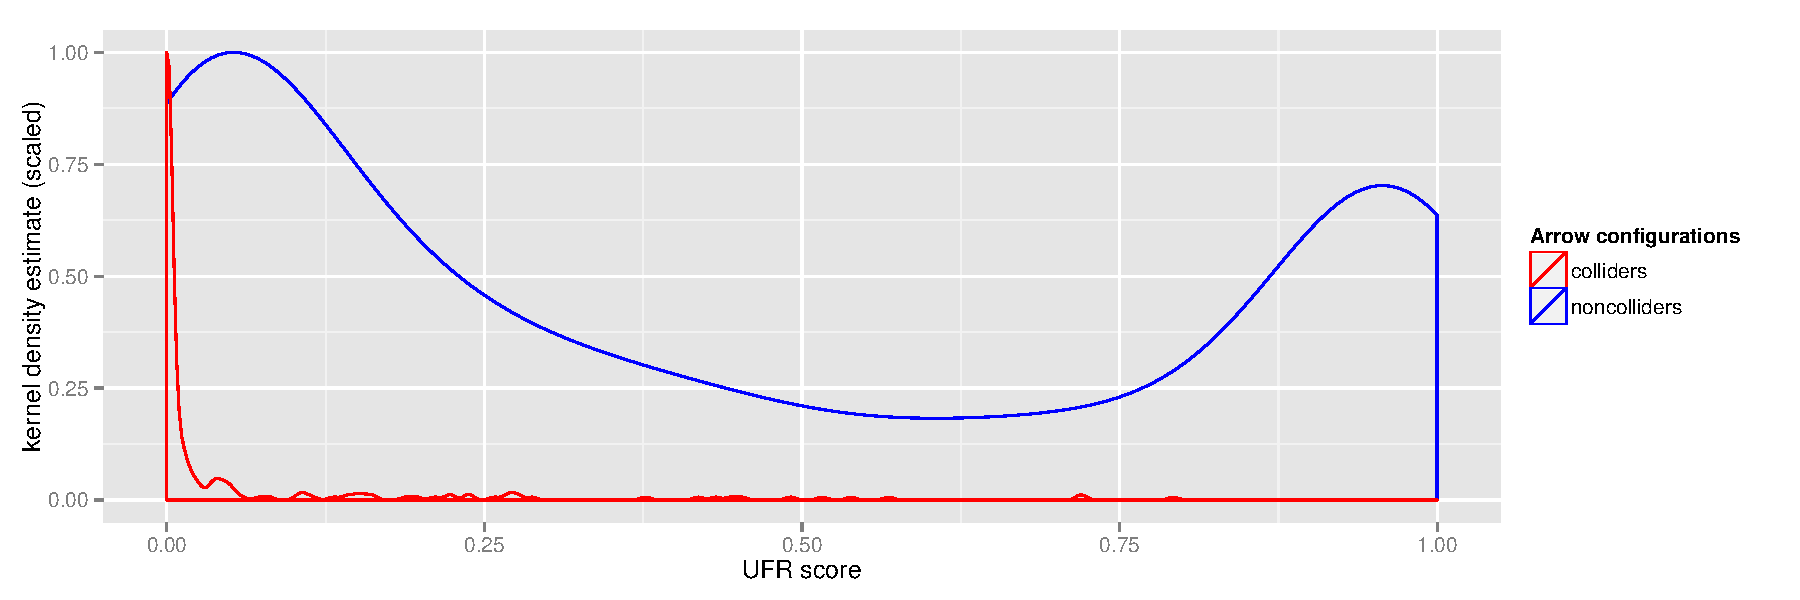
\includegraphics[width=\textwidth]{figures/ufr-density.pdf}
 \caption{UFR scores for collider and non-collider test instances}
 \label{ufr-scores}
\end{figure}

Analysing the precision-recall tradeoff on the $ufr$ values, the optimal threshold in terms of F-score was found to be as low as $0.004$. This is the value I chose to adapt, so that the test $ufr < 0.004$ constitutes the UFR criterion for v-structure detection. 

\subsection{Triangle Score Sum (TSS): aggregating directionality hints}
Another possibility to stabilize directionality inference is to move away from the framework of propagating binary v-structure decisions, instead embracing the fact that on noisy data, the different triples that each link in the skeleton takes part in may yield conflicting evidence of different strength. The obvious idea then is to quantify the directionality evidence present in each triple, and to combine these scores into an aggregate measure where conflicting evidence cancels out, and random spurious patterns in a single triple are overwritten by a larger number of more well-behaved triples. The basic quantification of directionality evidence in a triple can again be expressed in terms of the difference between the three-way overlap we observe, and the overlap we would expect in a non-collider.

If we continue to only consider the unshielded triples that are still present in the skeleton, and try to aggregate an evidence score from these measures, we are frequently faced with the problem that there is an unshielded triple only for one direction, or that there is a severe imbalance in evidence strength for both sides. This means that small errors in the skeleton can still propagate into large errors in directionality inference.

This leads to the idea of not considering only unshielded triples, but all sets of three languages in the dataset for deciding each link, making the directionality inference step independent from skeleton inference. The resulting score infers for every pair of languages in the entire graph whether a connection between them would look directional, based on the triangle scores of that pair with every other language.

In the discussion that follows, shorthands will be used to compactly represent the relevant overlap quantities. For the shared material between each pair of variables, we use the Greek letter corresponding to the member of the triple that is not involved, i.e.\ $\alpha := \frac{c(B,C)}{\min(c(B),c(C))}$, $\beta := \frac{c(A,C)}{\min(c(A),c(C))}$, and $\gamma := \frac{c(A,B)}{\min(c(A),c(B))}$.\\
In addition, I will use $\delta := \frac{c(A,B,C)}{\min(c(A),c(B),c(C))}$ for the amount of information shared between all three variables. In the notation, the hat diacritic will be used to denote expected overlaps, as opposed to observed values. I will be predicting the expected value $\hat{\delta}$ for the overlap based on the other observable overlap ratios, and then derive a quantification of the evidence against the assumed collider from the difference between observed $\delta$ and expected $\hat{\delta}$.

Let us now derive an approximate expression for $\hat{\delta}$ in the pattern $A \arrowLA B \arrowAL C$, which in the absence of latent variables is the only v-structure scenario. The only way in which a cognate set can come to be shared between all three languages in this scenario is if it was already shared between $A$ and $C$, and was borrowed into $B$ from one of the two languages. The percentage of material shared between $A$ and $C$ is given by $\beta$, and the percentage of material in $B$ borrowed from $A$ and $C$ is simply $\gamma$ and $\alpha$, respectively. Assuming independent sampling, the percentage of items which end up in $\delta$ via the transfer $A \arrowLA B$ should be equal to $\gamma \cdot \beta$, and the percentage transmitted via $C \arrowLA B$ should be $\alpha \cdot \beta$. When we simply add up these percentages, we will count some of the expected transferred items twice. The probability for each element in $cog(A,B,C)$ to have been selected twice is simply $\beta$, because this is the 
probability that a random element picked for transfer from $A$ or $C$ is shared by both nodes. We therefore expect $\delta \cdot \beta$ items to have been counted twice. Using this as a correction, we receive $\hat{\delta} = \gamma \beta + \alpha \beta - \hat{\delta}\beta$. Resolving this expression for $\hat{\delta}$, we arrive at the following equation for the expected three-way overlap in a collider:

\begin{equation*}
 \hat{\delta}(A \arrowLA B \arrowAL C) := \frac{\beta(\alpha + \gamma)}{1 + \beta}
\end{equation*}

Note that we considered the shielded case here. The situation of an unshielded triple is covered by $\beta := 0$, which causes the definition to collapse to $\hat{\delta} = 0$, capturing the intuition I already used in UFR, namely that a v-structure should result in zero three-way overlap that cannot be explained by other paths.

Turning the fitting of $\delta$ to $\hat{\delta}$ into a fit score could be done in a number of ways, but the easiest way turned out to be to form the quotient of the smaller by the larger of the two values, with special treatment for boundary cases to avoid division by zero:

\begin{equation*}
   ts(A \arrowLA B \arrowAL C ) :=
   \begin{cases}
     1 - \frac{\min(\delta,\hat{\delta}(A \arrowLA B \arrowAL C))}{\max(\delta,\hat{\delta}(A \arrowLA B \arrowAL C))} & \text{if } \delta > 0 \text{ or } \hat{\delta}(A \arrowLA B \arrowAL C) > 0\\
     0 & \text{if } \delta = 0 \text{ and } \hat{\delta}(A \arrowLA B \arrowAL C) = 0
   \end{cases}
\end{equation*}
\linebreak
$ts(A \arrowLA B \arrowAL C)$ measures the strength of evidence which the cognacy overlaps between the three languages provide against the v-structure pattern. Because all triangle scores are on the same scale, but cover overlaps of different strengths, we cannot directly add up these triangle scores to aggregate the directionality information they encode into a global evidence score. To avoid strong influences from languages with little overlap to the pair in question, it is necessary to weight the contributions to the triangle score sum by their relevance to the link in question. One simple way to define these weights is by considering the strength of the connection of the third variable $C$ to either of the two variables involved, and then normalizing these weights to keep the weighted sum in the $[0,1]$ range. In practice, making the weight differences a little more pronounced helped to moderate the contribution of distant third languages, leading me to square the weights before normalization:

\begin{equation*}
 w'(A \arrowLA B; C) = \max\left(\frac{c(B,C)}{c(B)},\frac{c(A,C)}{c(A))}\right)^2
\end{equation*}

The normalization of weights then happens in the obvious way:
\begin{equation*}
 w(A \arrowLA B; C) = \frac{w'(A \arrowLA B; C)}{\sum_{D \notin\{A,B\}} w'(A \arrowLA B; D)}
\end{equation*}

Finally, the weighted sum of triangle scores over all third variables $C$ gives us the definition of the \textit{\isi{Triangle Score Sum (TSS)}} after which the directionality inference method is named: 
\begin{equation*}
 tss(A \arrowLA B) = \sum_{C \notin\{A,B\}} w(A \arrowLA B; C) \cdot ts(A \arrowLA B \arrowAL C)
\end{equation*}

The TSS can be calculated on each link for arrows in both directions, and the results have the same scale, yielding a natural decision criterion in terms of the evidence strength quotient:

\begin{equation*}
 sc(A \arrowLA B) = \frac{tss(A \arrowLA B)}{tss(B \arrowLA A)}
\end{equation*}

\largerpage
To understand better how TSS works, let us take a look at an example from the Baltic Sea scenario. For the link betwen \ili{Russian} and \ili{Kildin Saami} (\iso{sjd}), the triangles with the heighest weight are given by \ili{Skolt Saami} (\iso{sms}), due to its high overlap with Kildin Saami, as well as by \ili{Polish} (\iso{pol}) and \ili{Belarusian} (\iso{bel}), both due to their high overlap with Russian. Together, these three triangles account for $62.3\%$ of the total weight sum, meaning that if a strong tendency arises from these three triangles, it will not be inverted by the remaining low-overlap triangles. Let us start with $ts($\iso{sjd} $\arrowLA$ \iso{rus} $\arrowAL$ \iso{bel}$)$. If this were a true v-structure, we would expect a three-way overlap of 34.55 cognates. In reality the overlap is higher at 47, giving a moderate counterevidence score of $ts($\iso{sjd} $\arrowLA$ \iso{rus} $\arrowAL$ \iso{bel}$) = 0.265$. From the reverse perspective, we have a much better fit at $ts($\iso{rus} $\arrowLA$ \iso{sjd} $\arrowAL$ \iso{bel}$) = 0.068$, because the prediction in this case would be an overlap of 50.42 cognates. The first triangle thus delivers a score contribution that is almost four times higher for the arrow direction \iso{rus} $\arrowLA$ \iso{sjd}. The scores for the other two triangles we consider point in the same direction: $ts($\iso{sjd} $\arrowLA$ \iso{rus} $\arrowAL$ \iso{pol}$) = 0.362$, but $ts($\iso{rus} $\arrowLA$ \iso{sjd} $\arrowAL$ \iso{pol}$) = 0.105$, and $ts($\iso{sjd} $\arrowLA$ \iso{rus} $\arrowAL$ \iso{sms}$) = 0.232$ is much higher than $ts($\iso{rus} $\arrowLA$ \iso{sjd} $\arrowAL$ \iso{sms}$) = 0.073$. From these three triangles, we can begin to approximate $tss($\iso{rus} $\arrowLA$ \iso{sjd}$) = 0.300 \cdot \frac{0.068}{0.265} + 0.165 \cdot \frac{0.105}{0.362} + 0.148 \cdot \frac{0.073}{0.232} + \dots \approx 0.2786$. The actual value with the full triangle sum is $tss($\iso{rus} $\arrowLA$ \iso{sjd}$) = 0.6658$, i.e. the missing triangles will equal the score out quite a bit, although the general tendency for more evidence against \iso{sjd} $\arrowLA$ \iso{rus} (i.e. a signal against the wrong directionality) remains.

The challenge of the TSS approach is to decide on a threshold for turning the evidence strength quotient $sc(A \rightarrow B)$ on each link into a directionality decision $A \arrowLA B$. For instance, is $sc(A \arrowLA B) = 0.667$, i.e.\ 50\% more evidence in this direction than the other, enough to make the decision? Reusing the five scenarios generated to derive the best $ufr$ threshold, I extracted the 211 links that were not part of the phylogenetic tree, of which 187 are monodirectional. For each link $A \arrowLA B$ I computed $sc(A \arrowLA B)$. If $sc(A \arrowLA B) < 1.0$, evidence pointed in the right direction, making this an instance where TSS worked correctly. Counterbalancing this are the cases where $sc(A \arrowLA B) > 1.0$, i.e. where the implied arrow was inverted. \figref{ufr-scores} shows the distribution of $sc(A \arrowLA B)$ for the good instances, and the inverse for bad instances. The separation is disappointingly bad, indicating that the possible advantage of a pairwise criterion like TSS over a triple-based like UFR is much reduced by the more difficult classification task. Still, it is clearly visible that the correct arrows tend to cluster closer to 0, and the inverted arrows closer to 1. This gives me an empirical basis for deciding on a threshold value, because I want as many good instances as possible below the threshold, while keeping as many bad instances as possible above it, because I prefer not assuming an arrow at all to inferring wrong directionality of contact.

\begin{figure}
 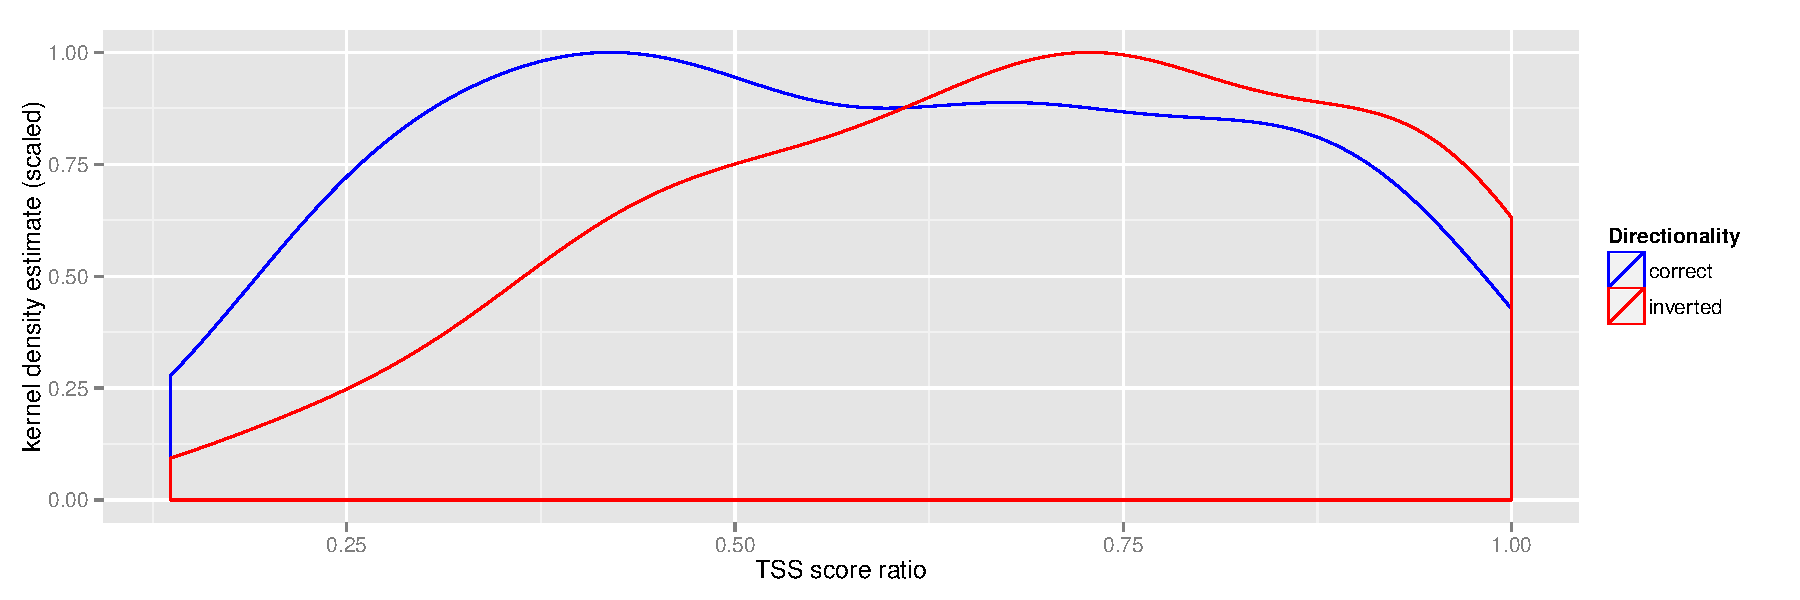
\includegraphics[width=\textwidth]{figures/tss-density.pdf}
 \caption{TSS scores for correct and inverted arrows}
 \label{tss-scores}
\end{figure}

This is another instance of a precision-recall tradeoff, where in addition to the correct and inverted TSS scores, the bidirectional links filter in as additional false instances in either direction. Aiming for a precision of 70\%, we can only get a recall of 21\% with a threshold value of 0.424. On the other hand, if we want to find two thirds of all arrows (66\% recall), we can only achieve that with a threshold of 0.982, i.e. we would have to add arrows very aggressively. A good compromise needs to be found somewhere between these values. Precision remains about constant at 64\%, i.e. about two thirds of inferred arrows are correct, across a very large range of threshold values between 0.555 and 0.720, which is when it starts to drop significantly. At the threshold value of 0.72, the maximum of this range, recall is at 47\%, which seems to be a reasonable compromise given the overall low performance.

In these considerations, we have not considered how the performance of TSS and UFR varies with the number of shared cognates defining each link, i.e. with data sparseness. Unavoidably, the rather simple TSS method can easily be misled by noisy or sparse data. My general impression is that TSS works considerably better on the NorthEuraLex data than the test cases suggest, possibly because the relevant contacts shaping real datasets tend to include large numbers of cognates. The evaluation will shed more light on this question, showing that the intuition is largely, but not always, correct.

\section{The phylogenetic guide tree}\label{sec:6.6}
As explained at the start of this chapter, in order to infer fully general evolutionary networks via causal inference, I will need to infer data for the proto-languages. To establish the proto-languages that need to be reconstructed, and as a guiding datastructure for the reconstruction, I need some phylogenetic tree over the attested languages as a starting point. A fully integrated system that starts with word lists and returns a lexical flow network as a result, would therefore include at least a rudimentary component for phylogenetic tree inference. As we have seen in \sectref{sec:2.5.2}, phylogenetic tree inference is already a very well-established field, and any of the methods discussed by \cite{felsenstein2004} can in principle be used for this purpose.

The purpose of my investigation is to compare the performance of different network inference variants on the best possible guide tree, and not to provide a fully integrated software package. My software implementation therefore requires the user to specify cognate sets over the input data, and some phylogenetic tree over the same languages, with branch lengths. This leaves it to the user to plug in cognate detection or tree inference algorithms of their choice, making it possible for my system to profit from future advances in these two subfields, although basic methods for a one-pass processing from word lists to lexical flow network will be provided as part of the release version of my software.

For my experiments on the simulated data from \chapref{sec:5}, I will simply use the binary tree created by the simulated language split events, together with the branch lengths defined by the times at which these events occurred. This tree is then reduced to the languages which still lived at the end of the simulation, first removing all the branches leading only to extinct languages, and then removing non-branching nodes in the resulting tree while maintaining consistent branch lengths.

For the NorthEuraLex data, I will use the expert tree defined by Glottolog, again reduced to only those leaves which are attested in the database. Adding branch lengths to this non-binary tree is one of only two places where I found it necessary to use existing phylogenetic inference tools. According to a suggestion by Gerhard Jäger, the inferred cognates were encoded as binary features and given to the IQ-Tree software \citep{nguyen_ea_2015} as input for inferring branch lengths on the unrooted Glottolog tree. For the output, the tree was re-rooted with Mandarin Chinese (\textit{cmn}) as an outlier. None of the family-internal branch lengths inferred by the selected model GTR2+FO+ASC+G4 seemed unplausible on inspection (see Appendix B.2 for a visualization), so that the resulting tree seems adequate as input for reconstruction methods.

\section{Deriving proto-language models}\label{sec:6.7}
If I want to be able to treat proto-languages as observed variables in the causal inference paradigm, I need to put some effort into deriving at least a good hypothesis about the presence or absence of each cognate class at each ancestral node in our phylogenetic tree. The idea essential to reconstruction then is to assume that the proto-language of some group of observable languages is most likely to have contained those cognate sets which are present in a large (and diverse) subset of its descendant languages.

This is very similar to the reconstruction of ancestral genomes in bioinformatics, from where we can take a variety of readily applicable algorithms. In addition to the mainstream ASR (Ancestral State Reconstruction) techniques in this tradition, I also present a naive threshold-based approach that will be used as a baseline. After evaluating the different methods on the simulated data, only the best two methods will be used to arrive at a usable reconstruction of ancestral cognacy in the NorthEuraLex dataset, and this reconstruction will be treated just like actual observations for phylogenetic network inference.

\subsection{Ancestral state reconstruction algorithms}
From the large number of ASR methods discussed in the literature, I will only sample a few very common and robust variants that are trivial to extend from nucleotides to cognacy data. The treatment of the methods cannot be complete, and I neither have the space to give examples of each reconstruction algorithm here, nor to provide the full algorithmic details for each method. Still, my explanations should suffice to provide the reader with correct intuitions about each method, and the formal statements are precise enough to completely describe the core features of any implementation.

\subsubsection{Naive threshold-based approaches}
For the initial experiment, I opted for a simple recursive criterion. For each node in the expert tree, it includes those cognate sets that are present in a majority (more than 50\%) of its immediate daughter languages. This implies we start at the observable languages and their cognate sets, and reconstruct upwards in the expert tree, arriving at the root language(s) in a single bottom-up pass through the entire tree.

If we introduce the notation $P(l = A)$ for the probability of cognate class $A$ being reconstructed for some concept in the language $l$ with children $l_1,\dots,l_k$, the \isi{majority-based reconstruction} can be written as a recursive formula
\begin{equation*}
   P(l = A) :=
   \begin{cases}
     1 & \text{if } \frac{1}{k} \sum_{i=1}^k P(l_i = A) > 0.5\\
     1 & \text{if } k = 0 \text{ and the word for the concept was assigned to class } A\\
     0 & \text{else }
   \end{cases}
\end{equation*}
\linebreak
This simple definition directly implements an important property of any useful reconstruction, namely that a word which was borrowed once at an intermediate stage and therefore now turns up in every language of a branch with many languages, will not end up in the proto-language if there is no other branch which also features a cognate. This usage of the tree to channel the information is superior to an even more naive criterion that would simply count the occurrences of each cognate class at the leaves under each ancestral node.

The main problem of this approach is of course that it tends to err very much on the safe side, as reconstruction stops as soon as there is a configuration of two subgroups for which different ancestral states are reconstructed, which occurs very often in real data. On the other hand, the few reconstructions this method arrives at tend to be extremely reliable. A threshold lower than 0.5 could be introduced for nodes which are more than binary-branching, but this would quickly lead to far too generous reconstruction.

\newpage 
In sum, threshold-based approaches can only be expected to show a very low performance, and do not offer many options to fine-tune them to the specific task. I will still use the majority-based approach as a baseline for comparison with more advanced alternatives.

\subsubsection{Parsimony-based approaches}
The most direct modern approach to ASR is based on maximizing parsimony, which can be seen as a formalization of Occam's razor, i.e.\ the principle of selecting the simplest hypothesis which explains all the data. In the context of ASR, parsimony can simply be described by the number of state changes which the model needs to assume. If we reconstruct the ancestral states in such a way that the number of mutations the model needs to assume is minimized, we are maximizing the parsimony of our reconstruction.

The standard algorithm for maximum parsimony is the \isi{Sankoff algorithm}, originally defined by \cite{sankoff1972}, which uses dynamic programming to keep track of the minimal number of replacement operations which needs to be assumed for smaller subproblems, and fills a table for each node, storing the total number of replacement operations which each state at that node would imply. For the current optimal solution in each cell, backpointers are stored which make it possible to reconstruct the configuration of ancestral states which led to the minimum number of replacement events for the entire problem. In my application, there are two useful variants of this basic Sankoff algorithm, which differ in whether we consider the presence of each cognate set as an independent character, or treat the different cognate sets for one concept as the different values of a single multistate character.

In the first version, which I will call \textit{\isi{multi-value MP reconstruction}}, a separate run of this basic Sankoff algorithm is performed for each presence-absence character, meaning that the table for each node only has two cells (one for presence, one for absence). Formally, each cognate set $A$ is reconstructed for the subset $L_A \subseteq L$ of all languages for which $\sum_{(l_i,l_j) \in E} 1_{l_i \in L_A, l_j \notin L_A}$ is minimal, under the condition that $l \in L_A$ holds for every language $l$ where the cognate set $A$ is attested, and $l \notin L_A$ for every language $l$ where it is not. In this version, it is possible that absence is reconstructed for all cognate sets, leaving a node without reconstruction, or that presence is reconstructed for more than one cognate set at a given node, hence the name I am using.

The second version, which I will call \textit{\isi{single-value MP reconstruction}}, reconstructs exactly one cognate set from the set of ancestral nodes, out of a set of candidates defined by the cognate sets occurring in the attested languages assigned to that phylogenetic unit. The Sankoff table has as many cells as there are candidate cognate sets. Formally, given a cost function $c(A,B)$ for the replacement of cognate sets (typically, $c(A,A) := 0$ and $c(A,B) := 1$ for $A \neq B$), this variant assigns a tuple of cognate sets $(A_1,\dots,A_n)$ to all the nodes $(l_1,\dots,l_n)$ such that that $\sum_{(l_i,l_j) \in E} c(A_i,A_j)$ is minimal, while keeping one set $A_j$ of the cognate sets  assigned to each attested language $l_j$ fixed.

The main problem of parsimony-based ASR is that different branch lengths cannot be accounted for. This exploits existing knowledge only suboptimally, since if one of two languages forming some phylogenetic unit is known to be more conservative (which would be reflected by a shorter branch length or a lower replacement rate in phylogenetic tree models), this will make it more likely that the ancestral set survived in this language, making it more informative for the reconstruction. A related more general problem of MP is that there will often be a large number of maximally parsimonious reconstructions, i.e.\ parsimony alone does not give us a sufficient decision criterion for finding a single reconstruction.

\subsubsection{Fully probabilistic approaches}
More recent approaches to ASR work in the maximum-likelihood (ML) paradigm. These fully probabilistic methods treat the discrete states $y$ at internal nodes as unknown parameters whose values need to be estimated given the data $x$ we observe. An obvious choice is the maximum likelihood estimator, which maximizes $P(y|x)$, the probability of different parameter values given the observed data, with the help of Bayes' rule:
\begin{equation*}
 P(y|x) = \frac{P(x|y)P(y)}{\sum_y P(y)P(x|y)}
\end{equation*}
While the denominator is hard to compute, it is independent of $y$ and is therefore irrelevant for maximizing the expression. Maximum likelihood estimation assumes that no prior information about plausible values $P(y)$ is available, which reduces the task of maximizing $P(y|x)$ to maximizing the likelihood $P(x|y)$ that we see the data given parameter values $y$. A good ML estimator will typically converge to the most likely value of $y$, although it is possible that other values of $y$ are almost as likely, and that the ML estimate $\hat{y}$ is even an outlier in the space of plausible parameter values. Still, ML estimates of model parameters provably maximize the agreement of the model with the data in many types of inference problems, given ML estimation a strong independent motivation outside the Bayesian paradigm.

In the application to ASR, optimization is based on an explicit parameterized evolutionary model $P_{ij}(\theta)$ which fully describes how each state $i$ is likely to evolve along a given phylogenetic tree, and thereby assigns a probability $P(x|y,\theta)$ to the observed data for each set of parameter values. If the evolutionary model is Markovian (the probability of each state change only depends on the parent state, not on earlier states), dynamic programming can be used to efficiently derive the internal states $y$ which maximize $P(x|y,\theta)$. For different applications, different evolutionary models are plugged into this basic paradigm.

Apart from the different evolutionary models, the main dividing line between approaches to ML-based ASR is in the method the optimal ancestral states at internal nodes are calculated. In the computationally simpler \isi{marginal reconstruction} as introduced by \cite{yang_ea_1995}, reconstruction of states at an internal node $A$ is done by re-rooting the tree such that $A$ becomes the root, and then computing the likelihoods for the different states at each node in a bottom-up fashion, summing over all possible combinations of states in the children $ch(A) = \{B_1,\dots,B_n\}$ down to the leaf nodes:
\begin{equation*}
 \hat{y}_A :=  \arg \max_i L_A(i),\ L_A(i) := \sum_{j_1,\dots,j_n} \prod_{k=1}^n P_{ij_k}L_{B_k}(j_k)
\end{equation*}
These values can again be computed by dynamic programming, meaning that the computation is only more time-consuming than the Sankoff algorithm by a factor linear in the number of ancestral nodes.

By contrast, in the more complex \isi{joint reconstruction}, the likelihood is jointly maximized over reconstructed values at all nodes, which is computationally a lot more demanding. Moreover, according to \cite{yang_ea_1995}, this variant is less suitable for retrieving optimal reconstructions at each ancestral node (because suboptimal local solutions can be necessary for an optimal global reconstruction), which leads me to disregard it as an option for the current application.

Implementing marginal reconstruction from stretch is non-trivial, and the implementation details of existing systems are not fully specified in the literature. This makes ML reconstruction the second of the two places in my infrastructure where it seemed more prudent to rely on third-party software instead of engineering my own implementation to behave exactly like a reference implementation. For marginal ML reconstruction, I am using a somewhat brittle interface from my Java code into the R package \texttt{phangorn} via system calls to \texttt{Rscript}, and a custom method on the R side for output in a Nexus format which can be read back into Java and mapped onto the original character information.

In analogy to multi-value MP reconstruction, \textit{\isi{multi-value ML reconstruction}} operates on binary characters which encode the presence or absence of each cognate set at each node. For non-attested nodes, the marginal reconstruction assigns probability values to each of the two values \texttt{0} (absence) and \texttt{1} (presence) of each character. If the probability of \texttt{1} at an ancestral node is above 50\%, the corresponding cognate set is reconstructed for the respective proto-language. This variant shares its basic properties with multi-value MP reconstruction. Ancestral nodes can remain without any reconstructed cognate set if for each cognate set character, the probability of the value \texttt{1} was below 50\%.

For \textit{\isi{single-value ML reconstruction}}, we only use one multi-state character for each concept, where each state encodes one of the possible cognate sets. The marginal reconstruction then produces a probability distribution over all the possible cognate sets at each ancestral node, and we only reconstruct the one with the highest probability. The behavior of the resulting method is again similar to single-value MP reconstruction in that exactly one cognate set will be reconstructed for each ancestral node. Due to limits in the \texttt{phangorn} implementation which are well-justified for its main field of application in biology, there is no support for ambiguity in the input data. This prevented me from modeling the synonyms in the NorthEuraLex data, so that the single-value ML reconstruction only builds on the first form in each list of concept realizations.

Maximum-likelihood methods for ASR work on a single phylogenetic tree with branch lengths, which is typically inferred by a different (often Bayesian) method. This can lead to problems because the likelihood of the individual tree hypothesis that the reconstruction is based on is usually quite low, and a reconstruction which takes more than a point estimate of plausible trees into account will be much more sound if computationally feasible.

To account for the uncertainty in the tree reconstruction, Bayesian methods which account for the uncertainty in both the ancestral characters and the tree structure have been developed. The hierarchical Bayes method by \cite{huelsenbeck_bollback_2001} is able to model uncertainty in the tree, branch lenghts, and the substitution model at the same time, but is reported to lead to very high uncertainty in the results. The advantages of this more accurate quantification of uncertainty are unclear in an application where only a single optimal reconstruction can be used. This and the prohibitive computational complexity associated with fully Bayesian methods justify confining myself to the simpler maximum-likelihood paradigm.

\subsection{Evaluation of ASR algorithms on simulated data}
It is easy to evaluate the different ASR methods on the simulated data. Let us act as if we lost the true configurations of all dead languages in the simulated set, and are left with a reduced version of the true tree which only contains the living leaves, plus the internal nodes which are necessary to keep the branching structure over these leaves. We can then feed the reduced true tree and the data from the leaves into the different reconstruction algorithms.

To compare the results, we return to the true data we discarded, and compute the percentage of bits (representing presence or absence of each cognate class) at the reconstructed nodes that correspond to the true values, as well as precision and recall on the level of reconstructed classes. Finally, we analyse the difference in reconstruction quality for proto-languages of different age, to find out whether one of the algorithms is more robust at higher time depths.

The following five previously introduced ASR methods were compared in this way:
\begin{enumerate}
  \item \textbf{Mjrty} (majority-based), i.e.\ using the naive criterion of reconstruction or presence in the majority of children
  \item \textbf{MPsgl} (single-value MP), i.e.\ using the Sankoff algorithm to reconstruct exactly one correlate set for each concept at each node
  \item \textbf{MPmlt} (multi-value MP), i.e.\ using the Sankoff algorithm to reconstruct a binary presence/absence value for each correlate set and concept
  \item \textbf{MLsgl} (single-value ML), i.e.\ using a marginal estimator on multistate characters, and selecting the most likely cognate set for each ancestral node
  \item \textbf{MLmlt} (multi-value ML), i.e.\ using a marginal estimator on binary presence/absence values, reconstructing the correlate set if presence is more likely than absence
\end{enumerate}

Running the different reconstruction algorithms and comparing the results on our 50 simulated linguistic histories, we get the numbers in \tabref{asr-overall-results}. The overall picture is clearly in favor of the MP and ML methods, but the differences between the two are not very pronounced. Only for the single-value variants, there is a clear advantage for ML over MP. For both MP and ML, the single-value variants shows higher recall than the multi-value variants, because they always produce some reconstruction even if evidence is not very strong, but this comes at a significant cost to precision. The very conservative majority method has the highest precision, but achieves this at a much higher cost to recall than the MLmlt method almost equalling it in precision. Overall, MLsgl is clearly the best method, as it achieves the highest recall by a significant margin, without compromising too much on precision.

\begin{table}
 \centering
 \begin{tabular}{cccccc}
  \hline \hline
  \# & Mjrty & MPsgl & MPmlt & MLsgl & MLmlt\\ \hline
  Accuracy & 0.9804 & 0.9774 & \textbf{0.9830} & 0.9803 & 0.9829\\
  Precision & \textbf{0.8463} & 0.5720 & 0.8199 & 0.6292 & 0.8255\\
  Recall & 0.3212 & 0.5874 & 0.4586 & \textbf{0.6289} & 0.4386\\
  F-score & 0.4656 & 0.5796 & 0.5882 & \textbf{0.6291} & 0.5813\\
  \hline
 \end{tabular}
 \caption{Performance of different ASR algorithms on simulated data}
 \label{asr-overall-results}
\end{table}

In order to check the suspicion that the differences between the algorithms might become more pronounced at higher time depths, where the few really difficult reconstructions are, we can evaluate the performance separately on proto-languages of different ages. \figref{asr-results-by-age} visualizes the performance of the five reconstruction methods across twenty different age ranges.

\begin{figure}
 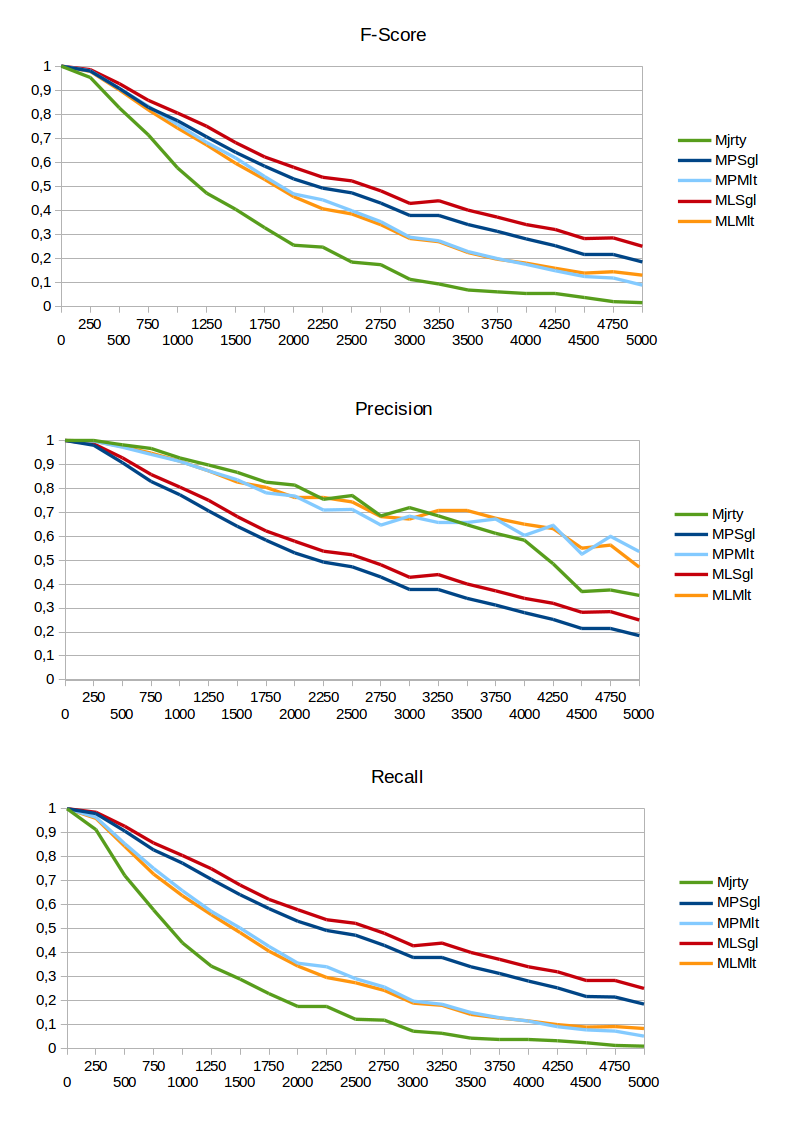
\includegraphics[width=\textwidth]{figures/recon-eval-timedepth.png}
 \caption{Development of ASR performance with age of reconstructed language}
 \label{asr-results-by-age}
\end{figure}

Whereas F-scores are satisfactory for reconstructed languages that go back only a few hundred simulated years, already at a time depth of 1,000 years substantial differences in the performance of the different algorithms start to appear. At higher time depths, recall becomes so low that the F-scores are already surprisingly close to zero. Still, there are some interesting developments at this highly problematic range. At a time depth of 5,000 years there is a clear split between three methods which essentially do not reconstruct anything useful any more (the majority method and the multi-state methods, all with recall under 10\%), and the other three methods which still manage to reconstruct at least some cognate sets (recall of 20-30\%), albeit with a high error rate (less than 40\% of the reconstructed cognate sets are correct). We can conclude that the acceptable overall performance of all methods in the previous analysis was mainly due to the dominance of simple reconstruction tasks if we evaluate across 
entire trees with many more younger languages than old ones. The task of reconstruction at higher time depths is still very much an unsolved problems. At these higher time depths, the two multi-state methods perform better precisely because they are biased towards assuming some reconstruction even if not enough evidence is available. However, since the overall advantage of the maximum-likelihood methods remains stable for proto-lan\-guages of any age, we at least know that they are clearly our best methods for phylogenetic flow inference, and will therefore be the default reconstructions used for the further experiments. The superiority of ML reconstruction over MP reconstruction was recently confirmed by \cite{jaeger_list_2017} on a different test set comprising real data from Indo-European, Austronesian, and Sinitic languages. In contrast to my simulated data, the performance of the methods is only evaluated against reconstructions at the level of the respective proto-language, i.e. at a high time depth. Just 
as in my experiment, the ML-single variant (ML-multi in their terminology) wins by a large margin.

\largerpage
\section{Phylogenetic Lexical Flow Inference (PLFI)}\label{sec:6.8}
Given a tree skeleton predetermined either by previous knowledge or inferred by means of a phylogenetic method, we can now apply ASR methods to derive cognate sets for the tree's internal nodes, and proceed to apply causal inference to the resulting dataset. Of course, this means that the performance of the method will hinge very much upon the quality of the reconstruction.

Very optimistically assuming that the output of our ASR method approximates the true history very closely, we treat all the nodes in our phylogenetic tree as observable languages, and apply lexical flow inference to a mixture of attested languages and reconstructed proto-languages. This is the algorithm which I propose to call \isi{Phylogenetic Lexical Flow Inference (PLFI)}.   \algref{plfi-algorithm} gives a description of all PLFI variants in pseudocode.

\begin{algorithm}\footnotesize
  \begin{algorithmic}[1]
  \STATE ASR method $asrM \in \{Mjrty,MPsgl,MPmlt,MLsgl,MLmlt\}$
  \STATE skeleton inference method $sklM \in \{PC,PS,FS\}$
  \STATE directionality inference method $dirM \in \{VPC,SPC,UFR,TSS\}\)
  \STATE $T := phyloInference(\{L_1,\dots,L_n\})$, or an expert tree
  \STATE $T := reduce(T,\{L_1,\dots,L_n\})$, the phylogenetic tree reduced to attested leaves
  \STATE $T := asr(T,asrM)$, add cognate classes to ancestral nodes by reconstruction
  \STATE $\mathcal{L} := nodes(T)$
  \STATE $G := (\mathcal{L},E) := (\mathcal{L},\{\{L_i,L_j\}\ |\ L_i, L_j \in \mathcal{L'}\})$, the complete graph
  \STATE $S \colon \mathcal{L} \times \mathcal{L} \rightarrow \wp(\mathcal{L})$, the separating set storage
  \STATE $s := 0$
  \WHILE{$s < |\mathcal{L}| - 2$}
    \FOR{$\{L_i,L_j\} \in G$ by increasing strength of remaining flow}
      \IF {$sklM \in \{PC, PS\}$}
        \FOR{each subset $S \in \wp(N)$ for neighbors $N$ of $L_i$ or $L_j$}
          \IF {$sklM = PC$ or all elements of $N$ are on paths from $L_i$ to $L_j$}
	        \IF {$|S| = s$ and $I(L_i;L_j|S) < 0.025$}
	          \STATE remove $\{L_i,L_j\}$ from $G$, $S(L_i,L_j) := S(L_i,L_j) \cup \{S\}$
	        \ENDIF
          \ENDIF
	    \ENDFOR
      \ELSIF {$sklM = FS$}
	    \FOR{each combination $P_1,...,P_k$ of paths from $L_i$ to $L_j$ of length $\leq 4$}
	      \IF {$|S| = s$ for $S := \bigcup\{P_1,\dots,P_k\}$}
	        \IF {ratio of $c(L_i,L_j)$ not explainable by flow across $S$ is $<$ 0.025}
		      \STATE remove $\{L_i,L_j\}$ from $G$, $S(L_i,L_j) := S(L_i,L_j) \cup \{S\}$
	        \ENDIF
	      \ENDIF
	    \ENDFOR
      \ENDIF
    \ENDFOR
    \STATE $s := s + 1$
  \ENDWHILE
  \IF {$dirM = TSS$}
    \FOR{$\{L_i,L_j\} \in G$}
      \IF{$sc(L_i \arrowLA L_j) < 0.72$}
         \STATE add arrow $L_i \rightarrow L_j$ to network
      \ENDIF
    \ENDFOR
  \ELSE
    \FOR{$L_i,L_j,L_k \in \mathcal{L}$ where $\{L_i,L_j\},\{L_j,L_k\} \in E$ but $\{L_i,L_k\} \notin E$}
      \IF{$(L_i \rightarrow L_j \leftarrow L_k)$ is a v-structure according to $dirM$ and $S(L_i,L_k)$}
	\STATE add arrows $L_i \rightarrow L_j$ and $L_k \rightarrow L_j$ to network
      \ENDIF
    \ENDFOR
    \STATE propagate arrows according to rules $\mathcal{R}_1$ to $\mathcal{R}_3$
  \ENDIF
  \RETURN network consisting of $G$ and arrows
  \end{algorithmic}
  \caption{PLFI($L_1,\dots,L_n$)}
  \label{plfi-algorithm}
\end{algorithm}

The PLFI algorithm requires either an expert tree, or a tree inferred by some phylogenetic tree inference algorithm, as input in addition to the cognacy data. After a preprocessing stage where the tree is reduced to the leaves for which data are available, some ancestral state reconstruction method (MLsgl by default) is applied to the tree and the data at the leaves in order to infer the presence or absence of each cognacy class at every non-leaf node in the reduced tree. The causal graph is then built over all the tree nodes.

The PC algorithm starts out with the fully connected graph, i.e. a network in which every pair of nodes is connected by a link. This graph is progressively thinned out to yield the skeleton by means of conditional independence tests based on separating set candidates. In each iteration, the algorithm increases the size $s$ of separating sets it considers. At each stage, it iterates through all the links remaining in the graph, and tries to build a separating set of size $s$ from the neighbors of the two languages it tries to separate.

Unlike in the vanilla PC algorithm, there is a defined order in which the links are tested for deletability. The PLFI algorithm always starts with the weakest remaining link, on the grounds that such links are more likely to arise due to random fluctuation in the noisy cognacy judgments. The links which represent the highest overlap are always checked last.

The separating set candidates which are tried out for the conditional independence tests depend on the skeleton inference method. If the skeleton inference method is set to $FS$, the flow-separation criterion introduced in \sectref{sec:6.4} is applied, so that every separating set candidate is composed of paths connecting the two languages in the current skeleton. Using one of the other skeleton inference methods, this first stage of the algorithm can also be configured to behave just like the vanilla PC algorithm or like PC*.

For the directionality inference stage, the user has the choice between four variants. The vanilla PC variant only differs from stable PC and the UFR criterion in the way in which v-structures are detected. In all three cases, the three standard directionality propagation rules of the PC algorithm are applied until all links are directed or none of the rules applies any longer. The only directionality inference method which works differently is the TSS-based variant, which infers the directionality on each arc separately by checking the TSS ratio against the threshold determined in \sectref{sec:6.5}. 


\section{Evaluation of PLFI}\label{sec:6.9}
There are two main ways to evaluate phylogenetic lexical flow inference which promise to be of interest. First, we can evaluate on perfect proto-data to determine the theoretical maximum performance the method could achieve if we had access to a perfect reconstruction. This gives us an upper bound on performance, because any real reconstruction will deviate from this perfect picture. To generate the input data for PLFI, we simply take the final state of the simulation for all languages, whether living or dead. This implies we include data from entire unattested lineages, including what we have earlier called para-languages and substrates, so that in this scenario, we have actual causal sufficiency, and the PC algorithm should be applicable without restrictions.

The more realistic evaluation of the method builds on reconstructed proto-data. Here, we reduce the known tree to ancestors of living languages, leaving only the lowest common ancestor in the cases were internal nodes become unary because one of two branches is deleted. Then, we apply one of the ASR algorithms to produce the data for the internal nodes of the reduced tree. To limit the number of cases to consider, we only evaluate on the two ML reconstruction methods which performed best on the simulated data, in order to be certain that our findings on simulated data carry over to the NorthEuraLex dataset.

\subsection{Evaluation metrics for phylogenetic flow}
Since causal inference as we employ it consists of the two stages of skeleton inference and directionality detection, for both of which we have multiple options at our disposal, it makes sense to first evaluate performance at the skeleton inference task, and then evaluate the different methods for directionality detection on the results of the best skeleton inference method.

For each connection $L_1 \arrowLL L_2$ which was found by the phylogenetic flow algorithm in the reconstructed network $G_{res}$, we can ask whether it corresponds to a lateral connection $L_1 \arrowLL L_2$ in $G_{true}$. If this is the case, we call the inferred connection a true positive ($tp$), otherwise a false positive ($fp$). If a lateral connection in $G_{true}$ does not have an equivalent in $G$, we count it as a false negative ($fn$). If for a pair of languages $L_1$ and $L_2$, neither graph has a connection $L_1 \arrowLL L_2$, we count it as a true negative ($tn$). From these four numbers $tp$, $fp$, $fn$, and $tn$, we can compute precision and recall, the standard measures of performance on binary classification tasks. The \textit{\isi{skeleton recall}} (SkRc) is then defined as $\frac{tp}{tp+fn}$, i.e the ratio of links in the true skeleton which the algorithm managed to reconstruct. Analogously, the \textit{\isi{skeleton precision}} (SkPr) can be written as $\frac{tp}{tp+fp}$, i.e.\ the ratio of 
links in the reconstructed skeleton which are correct. Both measures can be combined in a standard way via $2 \cdot \frac{SkPr \cdot SkRc}{SkPr+SkRc}$ to the \textit{\isi{skeleton F-score}} (SkFs), a combined performance measure which reaches high values if precision and recall are well-balanced.

For the evaluation on perfect proto-data, it is easy to adapt these standard performance measures, because there are no complications due to gaps in our knowledge which ASR cannot close. When evaluating on reconstructed proto-data, the situation is a little more complicated because some of the true connections cannot conceivably be found in the absence of substrates, and even in a perfect result, only the links between ancestors of related languages will be represented. For simulated contacts between pairs of languages where either only the donor or recipient of lexical material is in the input data (again, cases like substrate languages), we need to define which structures in the result graph would count as correctly reflecting reality, and which structures we would not accept as equivalent to the true story. In terms of precision, we will accept a link where either the reconstructed donor or the reconstructed recipient is the lowest ancestor of the true donor or recipient in the reduced tree, but not if 
both donor and recipient are wrongly detected, or contact is inferred between descendants. For each connection $L_1 \arrowLL L_2$ in the inferred network $G_{res}$, we therefore ask whether it is compatible with some connection in $G_{true}$, in the sense that it reflects a lateral connection $A_1 \arrowLL A_2$ for two languages $A_1 \in anc(L_1)$ and $A_2 \in anc(L_2)$ in $G_{true}$. For example, if a link \iso{isl} $\arrowLA$ \iso{eng} is found, we would accept it on the grounds of \proto{NorthGermanic} \arrowLA \iso{eng}.

While the definition of true positives and false positives remain rather straightforward in this way, the definition of false negatives becomes a bit more involved. Is \proto{NorthGermanic} $\arrowLA$ \iso{eng} captured by the inferred skeleton if it features a connection from any North Germanic\il{North Germanic languages} language to \ili{English}? Or should we require that all North Germanic languages should be connected to English by a lateral connection? Recall that the last option would require separate exclusive lexical flows of detectable size from every single North Germanic languages into English, which will typically not be possible. For this reason, I choose to relax the condition and only require the weaker representation. More formally, a link $L_1 \arrowLL L_2$ in $G_{true}$ which is not present in $G_{res}$ does not count as a false negative if there are descendants $D_1 \in des(L_1)$ and $D_2 \in des(L_2)$ in the phylogenetic tree such that $D_1 \arrowLL D_2$ in $G_{res}$.

With the skeleton in place, we can proceed to measure the quality of directionality inference on the links. The idea is to consider all correct links in the skeleton for which a directionality can be derived from the gold standard, and then analyse for which of these links the correct orientation was inferred. The fact that we actually have three possibilities for the gold standard ($\arrowLA$, $\arrowOA$, and $\arrowAA$), relative to which we have three possibilities for the result ($\arrowLA$, $\arrowAL$, $\arrowLL$), makes it a little less natural to define positives and negatives than for the skeleton measures. However, if we decide to count an arrow which points in the wrong direction as a false positive, and take the equivalence of $\arrowLL$ and $\arrowAA$ as well as the compatibility of $\arrowOA$ in the gold standard with both $\arrowLA$ and $\arrowLL$ in the result into account, we arrive at a plausible solution, which is defined by \tabref{arrow-eval-def}.

\begin{table}
\centering
\begin{tabular}{rlll}
  \hline \hline
  & $\arrowLA$ in result & $\arrowAL$ in result & $\arrowLL$ in result \\ \hline
  $\arrowLA$ in standard & \textit{true positive} + & \textit{false positive} + & \textit{false negative}\\ 
                                  & \textit{true negative} & \textit{false negative} & \\ \hline
  $\arrowOA$ in standard & \textit{true positive} & \textit{false positive} & \textit{true negative}\\ \hline
  $\arrowAA$ in standard & \textit{false negative} & \textit{false negative} & \textit{true negative}\\ \hline
\end{tabular}
 \caption{Table of elementary definitions for arrow evaluation}
 \label{arrow-eval-def}
\end{table}

\largerpage
Based on these elementary definitions, we can again define precision and recall measures in the standard way. Informally, the \textit{\isi{arrow recall}} (ArRc) then measures how many of the arrows in the gold standard on links in the derived skeleton also occur in the inferred network with the correct directionality. To complement this measure, \textit{\isi{arrow precision}} (ArPr) quantifies how many of the arrows in the reconstruction are justified by the gold standard. The trade-off between these two measures is of the same nature which one would typically capture in the precision-recall paradigm. If a directionality inference algorithm aggressively infers arrows even in the face of conflicting or weak evidence, this will increase arrow recall at the expense of arrow precision. A very cautious directionality inference scheme which assumes bidirectionality by default, will lead to a higher arrow precision at the cost of arrow recall. To handle this trade-off, we again mix both measures into the \textit{\isi{arrow F-score}} (ArFs) defined as $2 \cdot \frac{ArPr \cdot ArRc}{ArPr+ArRc}$, which will be our primary measure for comparing the performance of the different variants.

\subsection{Overall quantitative results for NorthEuraLex data}
Our first step for the evaluation is to compare the different methods in terms of skeleton precision and recall as well as arrow precision and recall on the entire NorthEuraLex dataset. This will allow us to choose the best method for the case studies in the next section.

\tabref{skeleton-evaluation-nelex} compares the skeleton precision and recall obtainable by the different conditional independence checks on our two maximum-likelihood reconstructions. While the single-value ML reconstruction led to the highest overall F-scores in the reconstruction experiments on simulated data, we find that the multi-value reconstruction consistently leads to better performance in all measures, especially in recall. These are the consequences of using the reconstruction with the highest precision, as this reconstruction will introduce the least noise, letting the patterns appear more clearly. The noise introduced by single-value reconstruction is so strong that it not only decreases the precision (leading to spurious lateral connections), but also the recall (letting weaker conditions disappear into the noise).

\begin{table}
 \centering
 \begin{tabular}{ccccccc}
  \hline \hline
   & \multicolumn{3}{l}{MLsgl reconstruction} & \multicolumn{3}{l}{MLmlt reconstruction}\\ 
   & PC & PS & FS & PC & PS & FS\\ \hline
  skPrc & \textbf{0.970} & 0.907 & 0.856 & 0.965 & 0.914 & 0.859\\
  skRec & 0.265 & 0.376 & 0.431 & 0.404 & 0.502 & \textbf{0.557}\\
  skFsc & 0.416 & 0.532 & 0.574 & 0.570 & 0.648 & \textbf{0.676}\\
  \hline
 \end{tabular}
 \caption{Comparing skeleton performance of MLsgl and MLmlt reconstructions on the NorthEuraLex data}
 \label{skeleton-evaluation-nelex}
\end{table}

\largerpage
The arrow performance measures are only defined for the intersection of links in the inferred skeleton and the gold standard, which will be a smaller or a larger set depending on the skeleton performance. Therefore, arrow performance cannot be reliably compared across reconstructions and skeleton inference variants. Still, we can compare the performance of the four directionality inference methods on the best skeleton. This is done in \tabref{arrow-evaluation-nelex}. As the results show, the two standard directionality inference methods used in the causal inference literature do not work at all, due to the non-exact conditional independence tests and the resulting difficulty to detect v-structures based on separating sets. On the multi-value reconstruction, the stable PC variant does not even manage to infer a single correct arrow. The two directionality inference methods introduced in this chapter fare a lot better, but there is an interesting contrast in their behavior on the different reconstructions. 
The single-value reconstruction gives an advantage to UFR, whereas TSS is clearly superior on the multi-value reconstruction.

\begin{table}
 \centering
 \begin{tabular}{ccccc}
  \hline \hline
   & \multicolumn{4}{l}{FS on MLsgl reconstruction}\\ 
   & VPC & SPC & UFR & TSS\\ \hline
  arPrc & 0.185 & 0.154 & \textbf{0.615} & 0.546\\
  arRec & 0.114 & 0.050 & \textbf{0.585} & 0.585\\
  arFsc & 0.141 & 0.076 & \textbf{0.600} & 0.565\\
  \hline
 \end{tabular}\\[0.5cm]
  \begin{tabular}{ccccc}
  \hline \hline
   & \multicolumn{4}{l}{FS on MLmlt reconstruction}\\ 
   & VPC & SPC & UFR & TSS\\ \hline
  arPrc & 0.240 & 0.000 & 0.410 & \textbf{0.500}\\
  arRec & 0.122 & 0.000 & 0.695 & \textbf{0.689}\\
  arFsc & 0.162 & (0.0) & 0.516 & \textbf{0.579}\\
  \hline
 \end{tabular}
 \caption{Comparing arrow performance of MLsgl and MLmlt reconstructions on the NorthEuraLex data}
 \label{arrow-evaluation-nelex}
\end{table}

Finally, to rank the different variants for overall performance, we can multiply the skeleton and arrow F-scores, capturing the intuition that the best approach should result in both a good skeleton and correct directionality information. The resulting numbers are given in \tabref{variant-comparison-nelex}, motivating our use of the MLmlt-FS-UFR variant for the case studies. Depending on the application, a different variant which is tuned towards more reliability at the expense of only finding the most prominent patterns, might be preferable. For applications where the focus is on precision (e.g.\ if computational means for deciding a research question are needed), the numbers on NorthEuraLex suggest that the MLsgl-FS-TSS variant might be the best option.

\begin{table}[t]
 \centering
 \begin{tabular}{lccc}
 \hline \hline
PLFI Variant & skFsc & arFsc & skFsc $\ast$ arFsc\\ \hline
\texttt{MLmlt-FS-UFR} & 0.6759 & 0.5793 & 0.3916\\
\texttt{MLmlt-PS-UFR} & 0.6477 & 0.5405 & 0.3501\\
\texttt{MLmlt-FS-TSS} & 0.6759 & 0.5157 & 0.3486\\
\texttt{MLsgl-FS-TSS} & 0.5736 & 0.6000 & 0.3442\\
\texttt{MLsgl-FS-UFR} & 0.5736 & 0.5647 & 0.3239\\
\texttt{MLmlt-PS-TSS} & 0.6477 & 0.4737 & 0.3068\\
\texttt{MLsgl-PS-UFR} & 0.5315 & 0.5455 & 0.2899\\
\texttt{MLsgl-PS-TSS} & 0.5315 & 0.5075 & 0.2697\\
\texttt{MLmlt-PC-UFR} & 0.5699 & 0.4333 & 0.2470\\
\texttt{MLmlt-PC-TSS} & 0.5699 & 0.3175 & 0.1809\\
\texttt{MLsgl-PC-UFR} & 0.4156 & 0.4242 & 0.1763\\
\texttt{MLmlt-PS-VPC} & 0.6477 & 0.2069 & 0.1340\\
\texttt{MLmlt-PC-SPC} & 0.5699 & 0.2105 & 0.1200\\
\texttt{MLmlt-FS-VPC} & 0.6759 & 0.1622 & 0.1096\\
\texttt{MLsgl-PC-TSS} & 0.4156 & 0.2424 & 0.1007\\
\texttt{MLsgl-PS-VPC} & 0.5315 & 0.1852 & 0.0984\\
\texttt{MLmlt-PC-VPC} & 0.5699 & 0.1714 & 0.0977\\
\texttt{MLsgl-PC-SPC} & 0.4156 & 0.2308 & 0.0959\\
\texttt{MLsgl-FS-VPC} & 0.5736 & 0.1408 & 0.0808\\
\texttt{MLmlt-PS-SPC} & 0.6477 & 0.1132 & 0.0733\\
\texttt{MLsgl-PS-SPC} & 0.5315 & 0.0889 & 0.0472\\
\texttt{MLsgl-PC-VPC} & 0.4156 & 0.1081 & 0.0449\\
\texttt{MLsgl-FS-SPC} & 0.5736 & 0.0755 & 0.0433\\
\texttt{MLmlt-FS-SPC} & 0.6759 & 0.0000 & 0.0000\\
  \hline
 \end{tabular}
 \caption{PLFI variants ranked by combined F-score on the NorthEuraLex data}
 \label{variant-comparison-nelex}
\end{table}


\subsection{Qualitative discussion of NorthEuraLex scenarios}
 To put some flesh on the performance measures on all of NorthEuraLex, we now turn back to the case studies discussed in \chapref{sec:4}. In the four following subsections, the lexical flow network inferred by the MLmlt-FS-UFR variant of the PLFI algorithm is given along with a second visualization which is color-coded for the difference to the gold standard.
 
 In the result graphs as in the gold standard, green arrows represent lateral connections for which directionality information could be inferred, and green lines mark lateral connections with conflicting evidence of directionality. In addition, yellow is used for links for which no causal evidence is available (typically isolated groups of two languages), and black arrows show the Glottolog tree which was part of the input, and remained an immutable part of the skeleton during all computations. The thickness of the lines symbolizes the unexplained cognacy overlap at the end of skeleton inference, i.e.\ the ratio of shared lexical material for which no other paths through the remaining graph exist. Evaluating these link weights in the lexical flow networks inferred by my algorithms would require a much more fine-grained gold standard which includes not only the contacts discussed in the literature, but a quantification of each contact's strength in addition. Some of this work was already done when compiling the gold standard, where some links will be left out because they did not seem to concern the subset of the lexicon covered by the database, but as we are going to see in the following discussion, even this simple pre-selection was not very successful. An evaluation of inferred contact strengths would therefore require a much more refined gold standard building on intersecting available lists of loanwords for many language pairs with the NorthEuraLex data, which will have to be postponed to future work.
 
 In the evaluation scheme I will use here, the evaluation graph symbolizes the fit of the inferred lexical flow network to the gold standard. It does not include link weights, but otherweise uses the same layout as the result graph, to which it adds red as well as additional dashed and dotted grey lines and arcs to highlight all types of errors in both the inferred skeleton and the inferred directionality information. The predefined phylogenetic tree backbone remains in black. Filled green arrows now stand for directional influences between related and unrelated languages that are compatible with the gold standard, whereas green lines symbolize lateral connections between related languages, which are always acceptable as possible artifacts because of imperfect phylogenetic trees or non-tree-like signals caused by dialect continua and similar phenomena leading to overlapping isoglosses. Empty green arrows represent links among related languages for which no directional contact is in the gold standard, but which are directional in the result.
 
 Other edge types encode various types of errors. Dotted light gray is used for false negatives in skeleton inference, i.e.\ lateral connections that were part of the gold standard, but are not found in the result graph. These arrows are kept rather unconspicious because the type of error they symbolize is arguably less problematic than the other categories. Spurious links (false positives in the skeleton inference) are dashed lines in dark gray, a pattern which is used for both arrows and undirected links between unrelated languages that are not justified by the gold standard. Finally, red is the color of the most problematic types of errors. Red lines with the empty diamond have the inverse direction to the one they should have according to the gold standard, whether among a pair of related or unrelated languages. Red lines are correctly inferred links which have a directionality in the gold standard, but are either bidirectional or undirected in the result. \figref{eval-graph-colors} summarizes the 
different edge types used in evaluation graphs for easier reference. Intuitively, evaluation graphs with large numbers of red connections indicate low performance, and a perfect network would only contain black and green (plus perhaps some dotted) connections.
 
 \begin{figure}
   \centering
   \fittable{
   \begin{tabular}{|ll|}
     \hline
     \begin{tikzpicture}[baseline=-0.5ex] \definecolor{tempcolor}{HTML}{000000} \draw[tempcolor,-Stealth,thick] (1,0.0) -- (3,0.0); \end{tikzpicture} & predefined arrow (defined by underlying tree) \\
     \begin{tikzpicture}[baseline=-0.5ex] \definecolor{tempcolor}{HTML}{339933} \draw[tempcolor,-Triangle,thick] (1,0.0) -- (3,0.0); \end{tikzpicture} & correct directed link across families (skeleton TP, arrow TP, arrow TN) \\
     \begin{tikzpicture}[baseline=-0.5ex] \definecolor{tempcolor}{HTML}{339933} \draw[tempcolor,-Triangle,thick] (1,0.0) -- (3,0.0); \end{tikzpicture} & correct directed link within family (skeleton TP, arrow TN) \\
     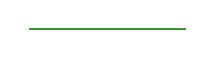
\begin{tikzpicture}[baseline=-0.5ex] \definecolor{tempcolor}{HTML}{339933} \draw[tempcolor,thick]    (1,0.0) -- (3,0.0); \end{tikzpicture} & correct undirected link (skeleton TP, arrow TN) \\
     \begin{tikzpicture}[baseline=-0.5ex] \definecolor{tempcolor}{HTML}{339933} \draw[tempcolor,-{Triangle[open]},thick] (1,0.0) -- (3,0.0); \end{tikzpicture} & spurious arrow within family (skeleton TP, arrow FP) \\
     \begin{tikzpicture}[baseline=-0.5ex] \definecolor{tempcolor}{HTML}{ee0000} \draw[tempcolor,-{Turned Square[open]},thick] (1,0.0) -- (3,0.0); \end{tikzpicture} & inverted arrow on correct link (skeleton TP, arrow FP, arrow FN) \\
     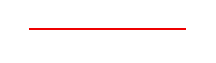
\begin{tikzpicture}[baseline=-0.5ex] \definecolor{tempcolor}{HTML}{ee0000} \draw[tempcolor,thick]    (1,0.0) -- (3,0.0); \end{tikzpicture} & missing arrow on correct cross-family link (skeleton TP, arrow FN) \\
     \begin{tikzpicture}[baseline=-0.5ex] \definecolor{tempcolor}{HTML}{808080} \draw[tempcolor,-{Triangle[open]},thick] (1,0.0) -- (3,0.0) [dashed]; \end{tikzpicture} & spurious directed link (skeleton FP) \\  
     \begin{tikzpicture}[baseline=-0.5ex] \definecolor{tempcolor}{HTML}{808080} \draw[tempcolor,thick]    (1,0.0) -- (3,0.0) [dashed] ; \end{tikzpicture} & spurious undirected link (skeleton FP) \\     
     \begin{tikzpicture}[baseline=-0.5ex] \definecolor{tempcolor}{HTML}{c0c0c0} \draw[tempcolor,-{Triangle[open]},thick] (1,0.0) -- (3,0.0) [dotted] ; \end{tikzpicture} & missing directed link (skeleton FN) \\
     \begin{tikzpicture}[baseline=-0.5ex] \definecolor{tempcolor}{HTML}{c0c0c0} \draw[tempcolor,thick]    (1,0.0) -- (3,0.0) [dotted] ; \end{tikzpicture} & missing undirected link (skeleton FN) \\
     \hline
   \end{tabular}
   }
   \caption{Summary of combined color, line style and shape coding used in evaluation graphs}
   \label{eval-graph-colors}
 \end{figure}
 
 After a quick summary of the result for each case study, I will mostly focus on individual cases of red and spurious links, and go into the details of the computation to elucidate why this variant of PLFI failed on these links. These investigations will help to get a full picture of why PLFI is not a perfect method, and lead to some ideas for possible future improvements beyond the current state.
 
 \subsubsection{Case study 1: the Baltic Sea area}
  \begin{figure}
 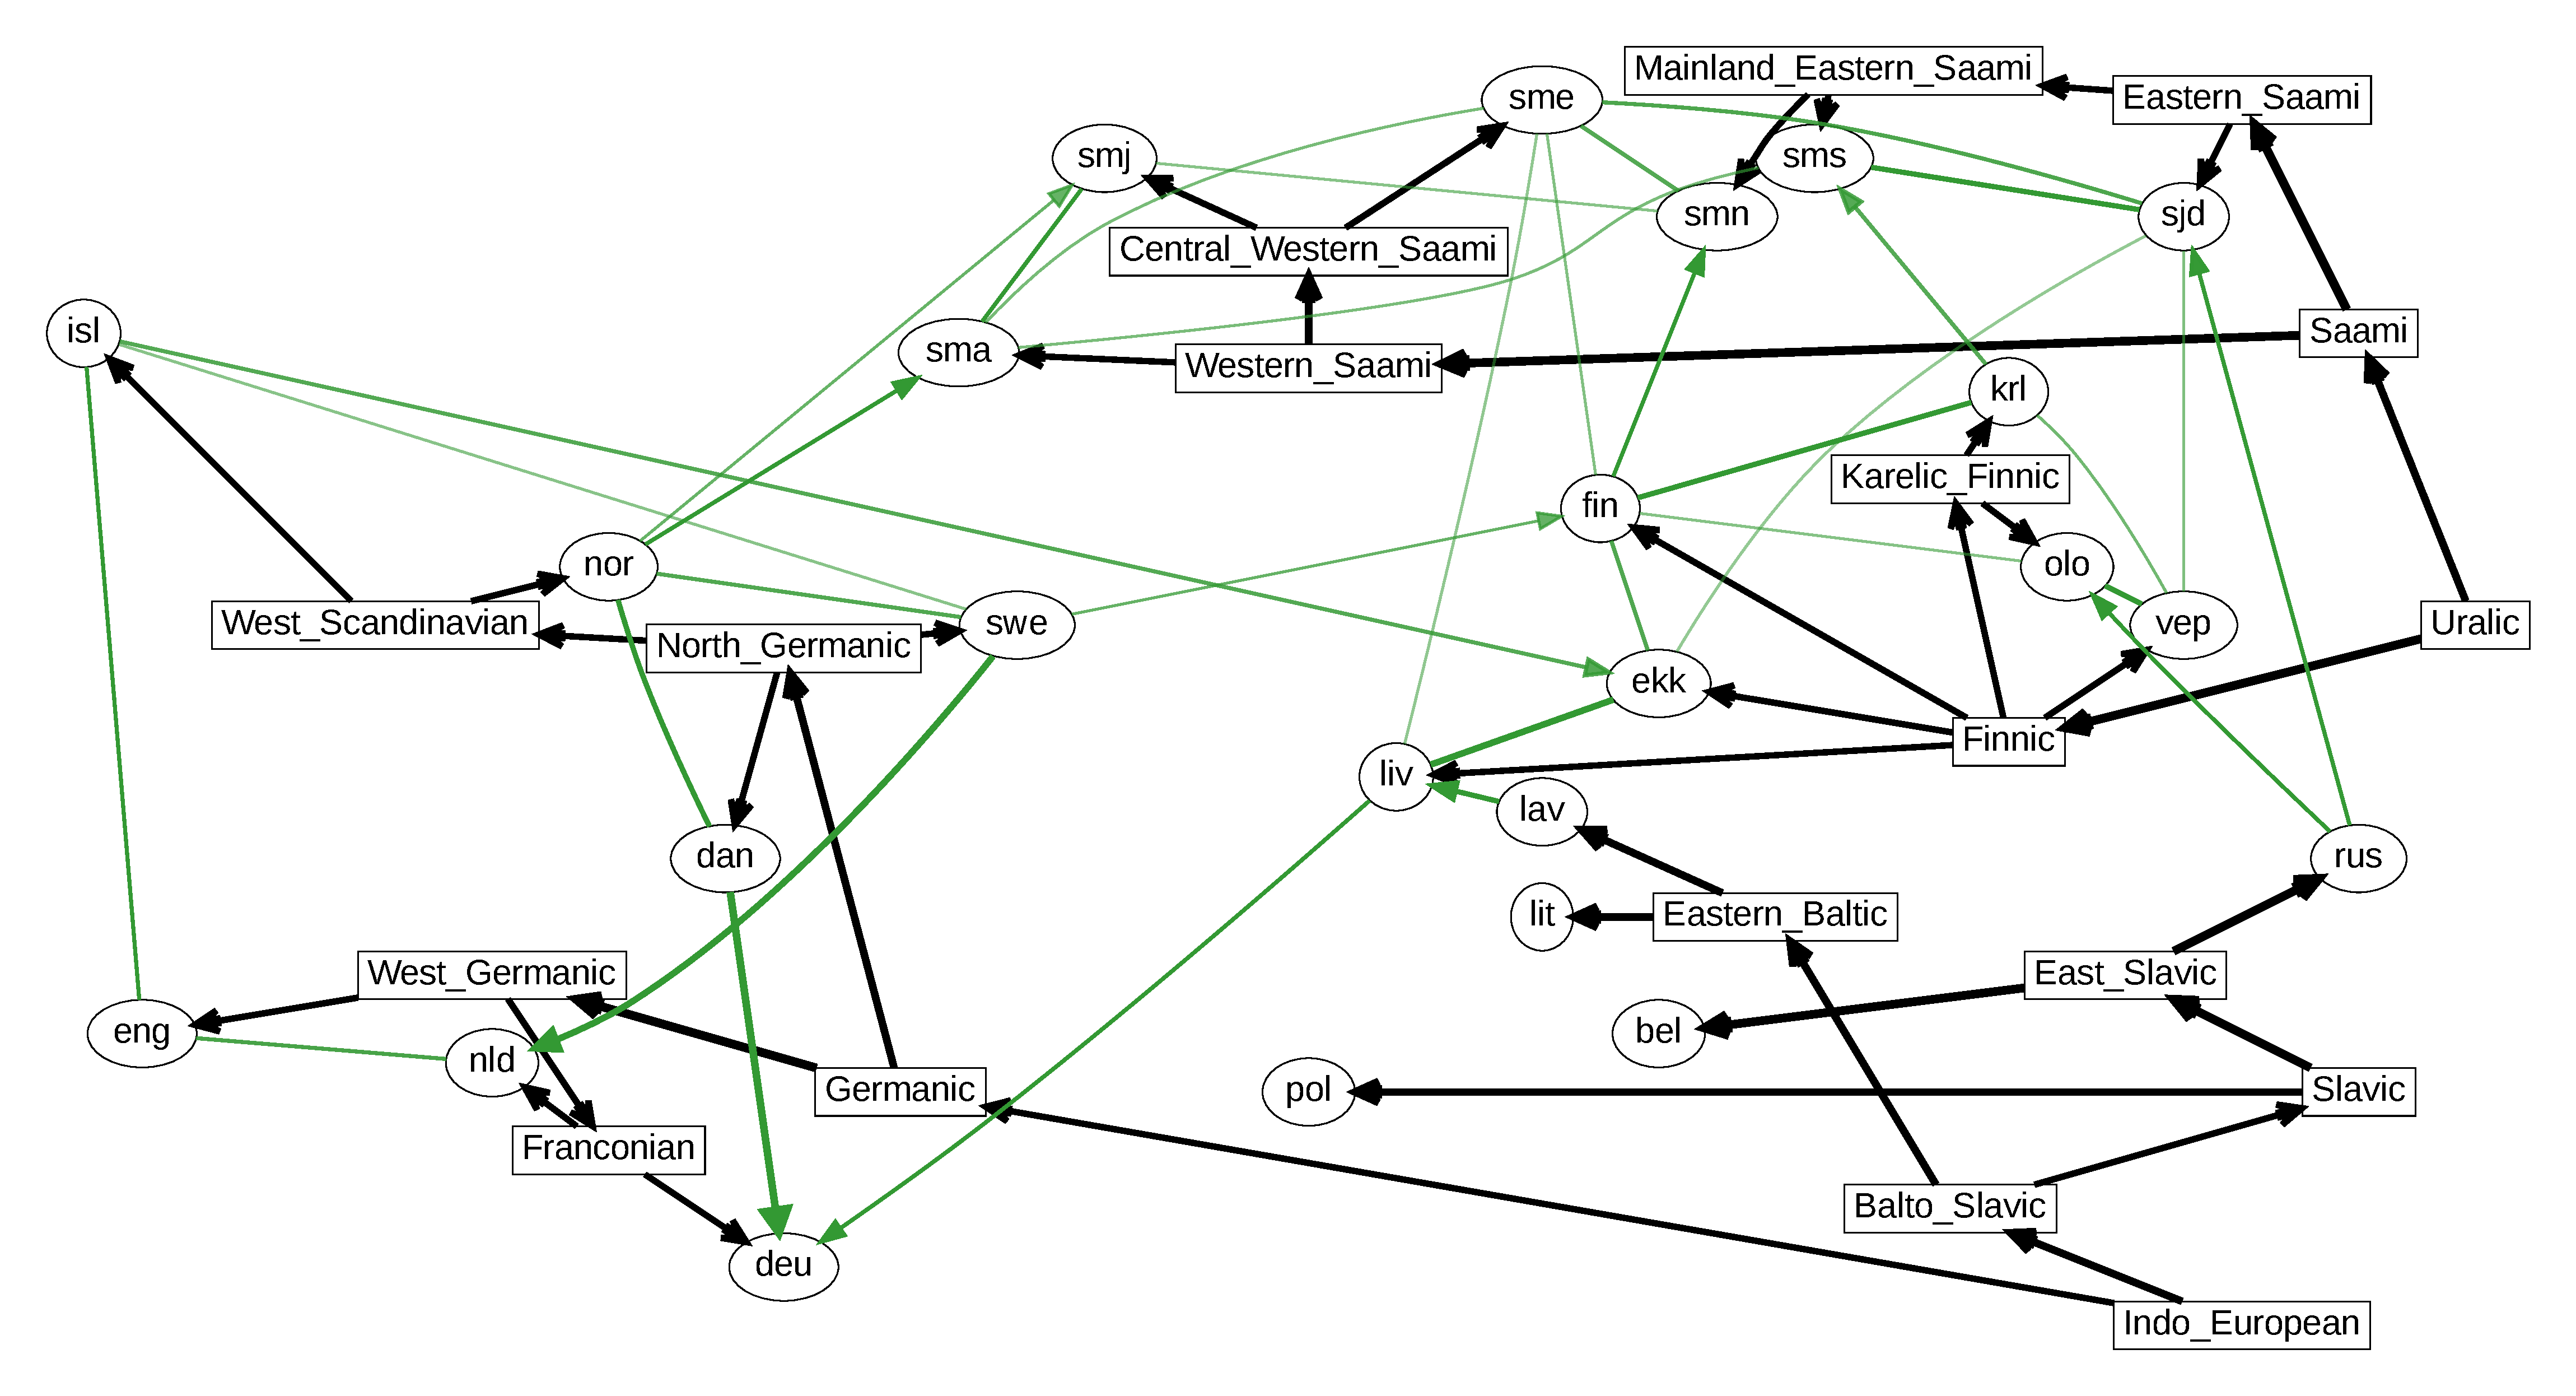
\includegraphics[width=\textwidth]{figures/baltic-fs-ufr-ml-multi.pdf}
 \vspace*{5mm}
 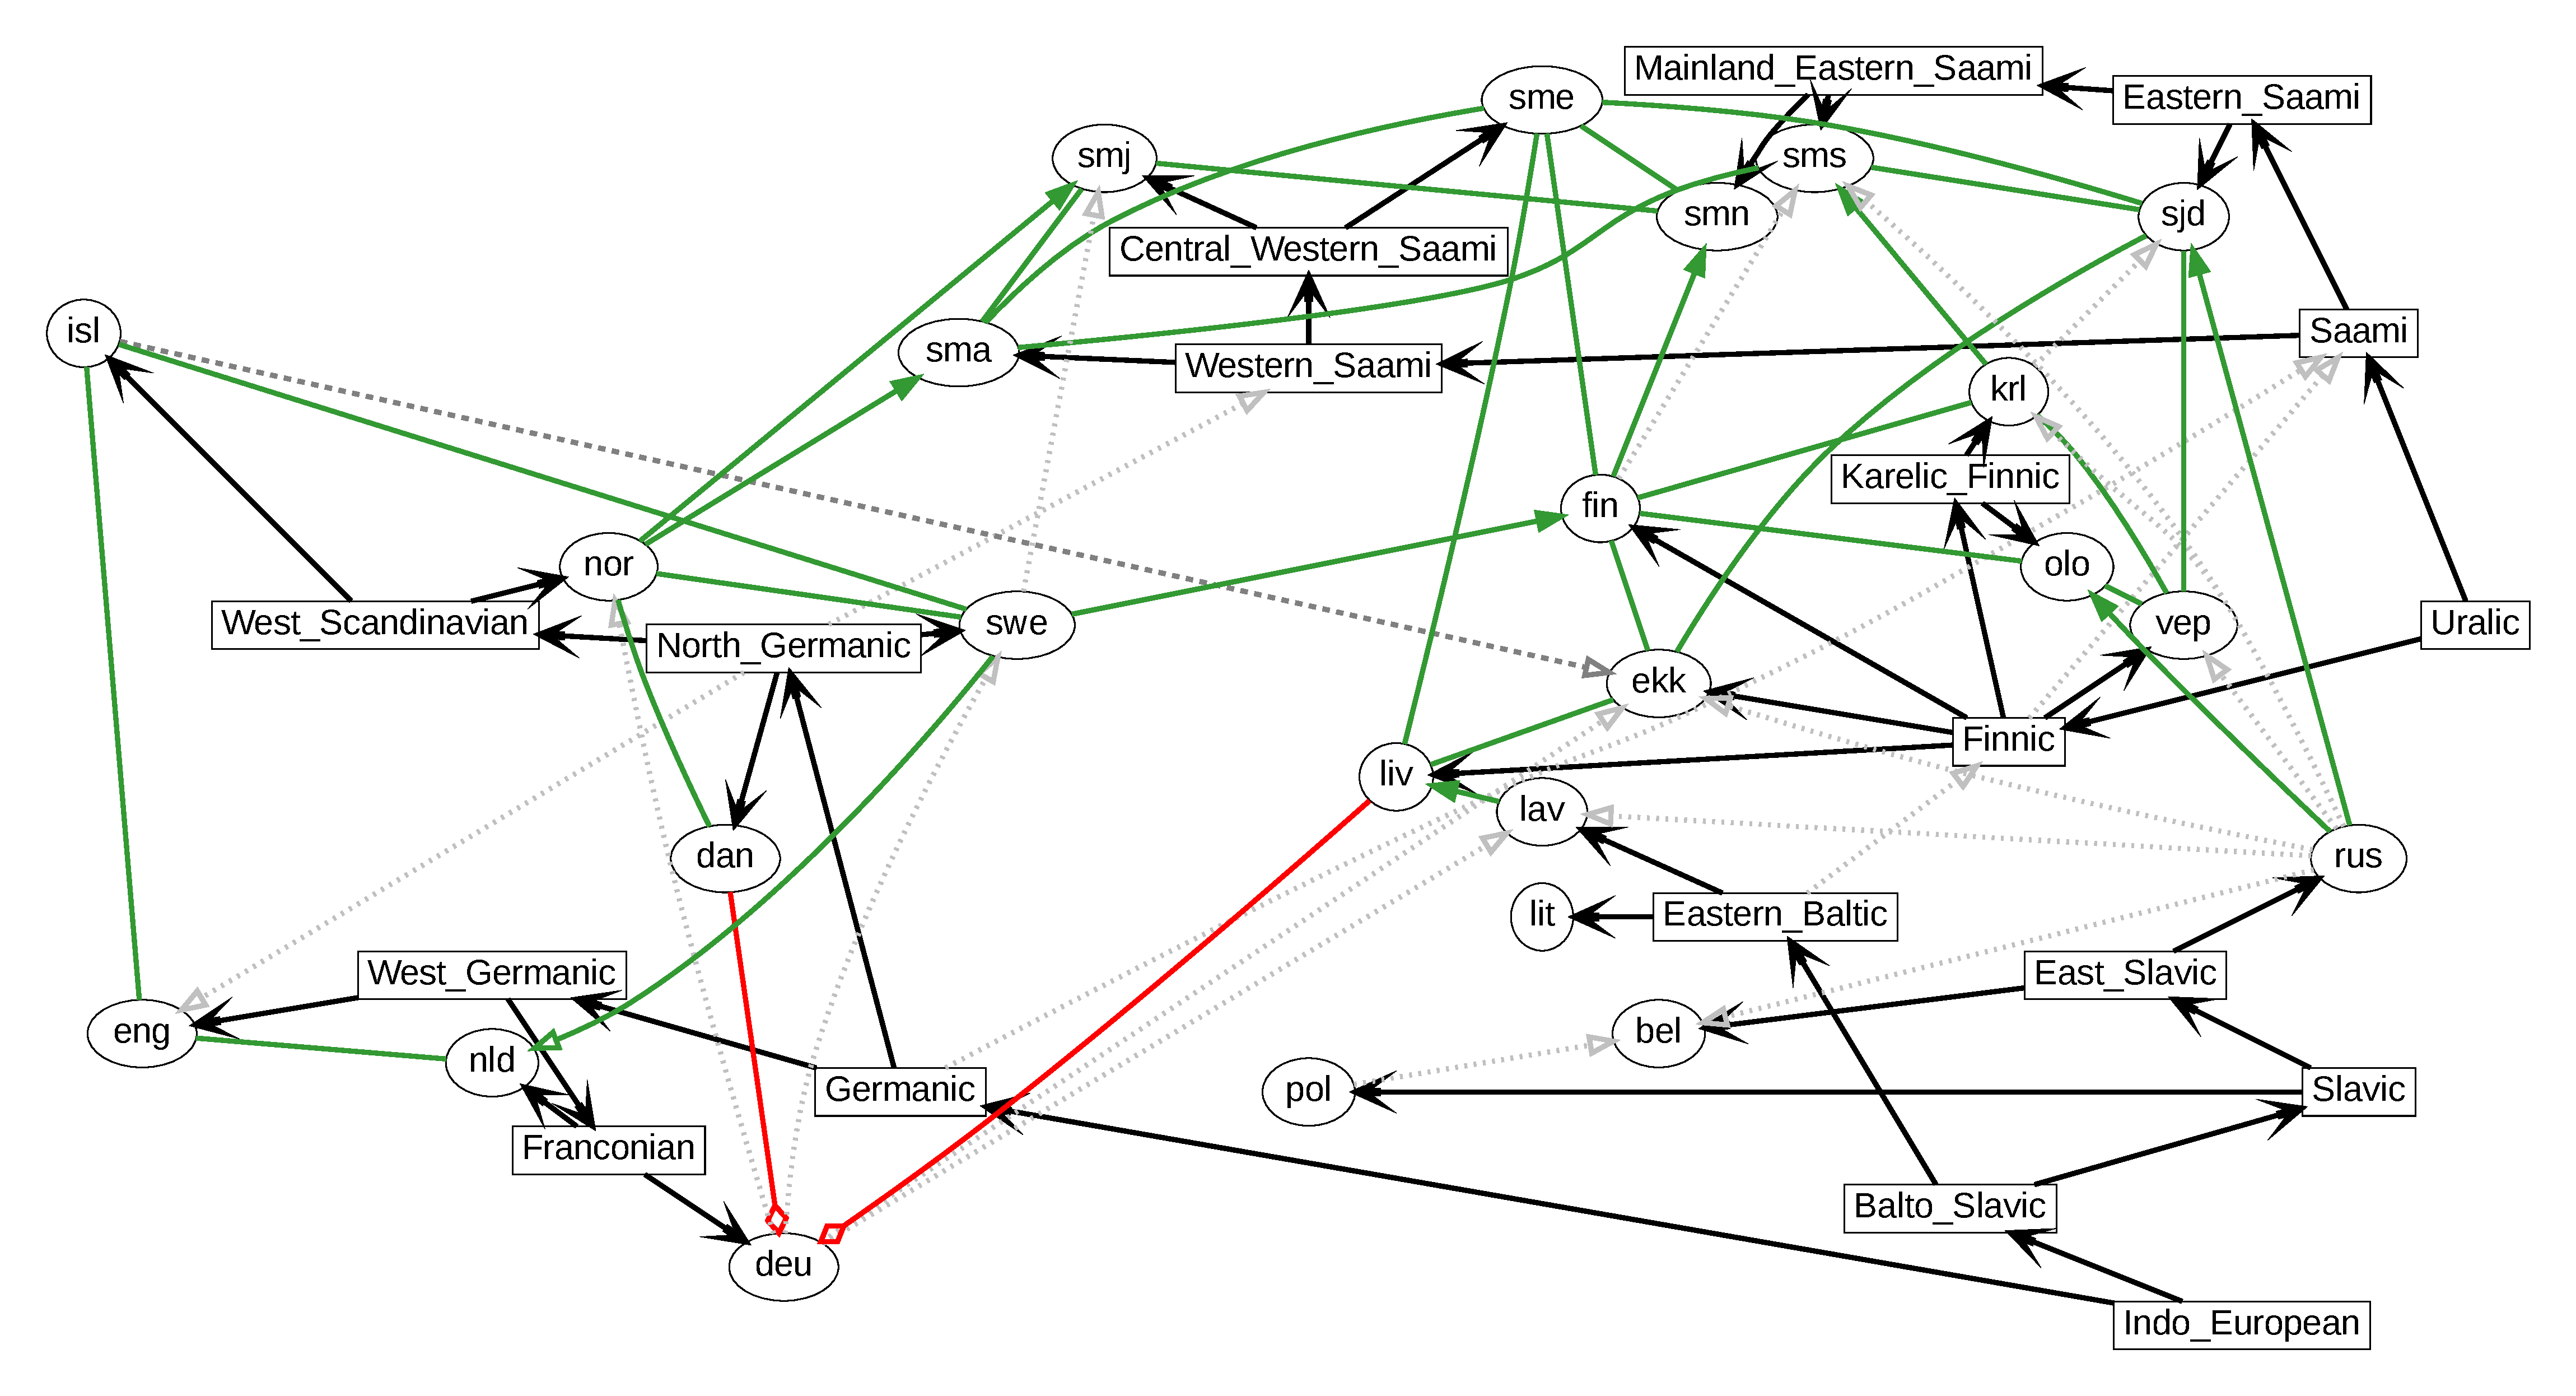
\includegraphics[width=\textwidth]{figures/baltic-fs-ufr-ml-multi-eval.pdf}
 \caption{Result graph (top panel) and evaluation graph (bottom panel) of phylogenetic flow on Baltic Sea data}
 \label{baltic-result-phylo}
 \end{figure}
 Already at first glance, the visualization of results for the Baltic sea case in \figref{baltic-result-phylo} displays only very few errors. The major contacts in the area are all inferred successfully: North Germanic\il{North Germanic languages} influence on Western Saami\il{Western Saami languages} (here imperfectly represented as influence from \ili{Norwegian} on the individual languages), \ili{Russian} influence on all the minority languages on its territory (invisible in the cases of \ili{Veps} and \ili{North Karelian}, due to the mentioned purism of the sources), \ili{Swedish} influence on \ili{Finnish}, and \ili{Latvian} loans in \ili{Livonian}.
 
 \newpage 
 Some other influences in the gold standard, such as the Baltic\il{Baltic languages} influence on Finnic\il{Finnic languages} and the Finnic influence on Saami\il{Saami languages}, were not visible in the data, most likely because the multi-value reconstruction these results are based on did not project sufficiently many cognate sets to the level of these proto-languages. This is something we will observe in many cases, due to the cautious reconstructions in this paradigm. Only in graphs derived from single-value reconstructions do the numbers of cognate sets in the ancestral languages become so high that influences between them cannot be explained away completely by their descendants.
 
 Other contacts in the gold standard are imperfectly represented by undirected lateral signals, such as the \ili{German} influence on the continental Scandinavian languages. This is represented by an inverted link from German to \ili{Danish}, whose close relationship with \ili{Norwegian} is recognized, but not as directional, and a second lateral connection involving \ili{Dutch} and \ili{Swedish}. This part of the skeleton could hint at a problem with the language sample in this case study, since much of the German material in Danish and Swedish was actually borrowed from \ili{Low German}, an unobserved language the closest relative to which in our dataset is Dutch. A different problem causes the spurious link from \ili{Icelandic} into \ili{Estonian}. This should actually be another link from German, the Germanic language which by far had the largest lexical influence on Estonian. Now the problem is that some of the material shared with German can be inferred as having flowed through \ili{Livonian}, which contains an even larger share of German loanwords. Some other Germanic words which cannot have travelled via Livonian are present in rather archaic forms in Icelandic, causing most cognates for the remaining overlap to be detected for that language instead of other Germanic languages.
 
 The wrong directionality of the arrow from \ili{Danish} into \ili{German} is simply due to the fact that the unshielded triple \iso{dan} $\arrowLL$ \iso{deu} $\arrowLL$ \proto{Franconian} is detected to be a v-structure due to a very low UFR score of 0.0013. This erroneous low score is due to high overlap of 461 words between Danish and reconstructed Franconian, of which not a single item can be explained only by paths going through German. This is due to the existence of alternative routes, one through inheritance from Germanic, and the other through the Dutch-Swedish connection. We thus have a case where the logic of UFR breaks down due to the complex interplay of path configurations.
 
 Coming to the final inverted arrow \iso{liv} $\arrowLA$ \iso{deu}, here it is the unshielded triple \iso{lav} $\arrowLL$ \iso{liv} $\arrowLL$ \iso{deu} which does not look like a v-structure at all. This triple has a very high UFR score of 0.6364, caused by the fact that out of the 22 items shared exclusively by \ili{Latvian} and \ili{German} (mostly German loans in Latvian), 21 are also shared by \ili{Livonian}. From the pattern \iso{lav} $\arrowLA$ \iso{liv} $\arrowOO$ \iso{deu} which arises after Latvian influence on Livonian was successfully detected, the propagation rule infers the erroneous link \iso{liv} $\arrowLA$ \iso{deu} because otherwise a previously rejected v-structure would have to be assumed. To interpret the result, to the flow model Livonian very much looks like a transmitter of Latvian words into German, after having explained away the contact link from German into Latvian demanded by the gold standard.
 
 To sum up, the two serious mistakes that were produced for this scenario are caused by the fact that the UFR-based v-structure test is not as reliable as it would have to be to guarantee a correct result. As always in constraint-based causal inference, even a single erroneous v-structure test can have strong effects due to propagation. Interestingly, the alternative method TSS has no problem at all to assign the correct directionality to the arrows involving German, once more showcasing the motivation for the alternative method. Since the TSS method makes other mistakes, a way towards avoiding inverted arrows (the worst type of mistake) could be to aggregate the results of both methods, only returning the arrows on which all directionality inference methods agree.
 
 \subsubsection{Case study 2: Uralic and contact languages}
 Moving on to the second case study, we see in \figref{uralic-result-phylo} that while there are a few more problematic arrows, the overall results are still rather convincing. Since the Western part of this case study was already covered by the previous experiment, I will not comment further on the Baltic Sea area here, except for one interesting point. In the absence of \ili{Dutch} from the language set, the West Germanic\il{West Germanic languages} material present in \ili{Swedish} is now inferred as being shared with Standard \ili{German}, the only West Germanic language remaining in the dataset. This highlights one property of the inference method: if relevant languages are not part of the dataset, the method will find the most plausible explanation involving only the attested languages and their recontructed ancestors. The addition or removal of one language can have consequences beyond the immediate vicinity of the language in question, due to alternative routing of lexical flow and changed propagation patterns for directionality information.
 
 Moving to European Russia, we see that the most dominant trend of the region, the pervasive influence of \ili{Russian} on many of the minority languages of the Russian Federation is inferred correctly (dark green arrows pointing outwards from \iso{rus}). The spurious arrows mainly concern inferred secondary influences between branches of Uralic\il{Uralic languages}, on which there is often no consensus among scholars, and which are therefore not represented in my gold standard. For instance, the inferred influence of \ili{Komi} (\iso{koi}) on \ili{Khanty} (\iso{kca}) is not implausible at all, and neither is Khanty influence (\iso{kca}) on \ili{Mansi} (\iso{mns}). On the other hand, most of the long-distance arrows are clearly spurious, such as influence of \ili{Estonian} (\iso{ekk}) on \ili{Hungarian} (\iso{hun}), and of \ili{Erzya} (\iso{myv}) on Mansi (\iso{mns}). Let us inspect a third example, the reconstructed secondary influence of \ili{Udmurt} (\iso{udm}) on \ili{Nganasan} (\iso{nio}), more closely. The reason why the link remains during skeleton inference is legitimate: there is some material shared between Samoyedic\il{Samoyedic languages} and the \ili{Permian languages}, but not the rest of Uralic. The reason why Nganasan and Udmurt were selected to model these lexical isoglosses is again due to the imperfect nature of the cognate detection. All the other Samoyedic languages have undergone much more disruptive sound change than Nganasan, causing the system to find more cognates between the more conservative Nganasan and the other Uralic languages. To a lesser extent, the same pattern applies on the Permian side, where Udmurt has undergone fewer sound changes than Komi. Finally, the erroneous arrow is caused by the fact that according to the UFR criterion, the Erzya (\iso{myv}) lexicon does not look like a mixture of Russian and Udmurt, and neither does Udmurt form a v-structure with Erzya and Nganasan, causing the arrow from Russian into Erzya to be propagated by the principle of avoiding additional v-structures.
 
 While a connection of \ili{Romanian} (\iso{ron}) with \ili{Bulgarian} (\iso{bul}) is inferred correctly by skeleton inference, the directionality of influence between the two languages is inferred to be the opposite of the real situation, where the Romanian lexicon is an obvious mixture of Slavic and Romance elements. The problem here is that Romanian is the only Romance language\il{Romance languages} in the dataset, meaning that on the reduced skeleton, the mixed character of the Romanian lexicon would have to be detected from a v-structure \proto{Indo-European} $\arrowLA$ \iso{ron} $\arrowAL$ \iso{bul} with Bulgarian or some other Slavic language\il{Slavic languages}. The UFR score for this triangle is rather close to zero at 0.0340, but not close enough for our empirically determined threshold. An additional Romance language in the dataset would yield a much cleaner v-structure \proto{Romance} $\arrowLA$ \iso{ron} $\arrowAL$ \iso{bul}, whereas too little of the Romance material in \iso{ron} can be reconstructed for \proto{Indo-European}.
 
 A second interesting area where some problems of the method become visible is the interaction between the Turkic\il{Turkic languages} and Uralic languages of the Volga region. The inferred network displays some shared material between \ili{Chuvash} (\iso{chv}) and the two \ili{Mari languages} (\iso{mrj} and \iso{mhr}), but cannot decide on the directionality of either connection. According to the gold standard, there should be arrows from Chuvash into both Mari languages, but this presupposes that \iso{mrj} $\arrowLA$ \iso{chv} $\arrowAL$ \iso{mhr} is not a v-structure. Unfortunately, a v-structure is exactly what we get by the UFR criterion, since on the rather dense skeleton, transmission via \iso{chv} is not needed to explain even a single item shared between \iso{chv} and both variants of Mari, as all of these are projected up to Proto-Mari. Here, the fact that local criteria are used is really showing its negative consequences, because nothing forces the model to explain how this Turkic material ended up in Proto-Mari, which is independent of any Turkic influence conditioned on its two descendants.
 
 A larger part of the Turkic element in \ili{Meadow Mari} (\iso{mhr}) is wrongly attributed to influence from \ili{Bashkir} (\iso{bak}), as it is correctly inferred for \ili{Udmurt}. As the orange color indicates, this is a problem of skeleton inference. Here, the reasons can be traced back to the fact that cognacy data are too coarse-grained to distinguish between different closely related donor languages. While Chuvash and Bashkir are not very closely related, their divergence has primarily happened on the phonetic level, which is not visible in the inferred cognacy data. Taking a look at the actual forms, it instantly becomes clear that Chuvash has been the main source of Turkic material in Mari, but this fact is hidden by the cognate set abstraction. A future improved measure of conditional mutual information which is computed from phonetic distances (see \sectref{sec:6.1.1}) could prove superior here.
 
 While skeleton inference performed with good overall precision, the one truly inexplicable link remaining in the inferred skeleton is the connection between the Balto-Slavic and Samoyedic proto-languages. Inspecting the cognate sets the distribution of which is explained by flow on the spurious link, we see that it mainly consists of Balto-Slavic cognate classes for concepts like \textsc{apple} and \textsc{cat}. As Russian loanwords, these cognate classes are also present in a majority of \ili{Samoyedic languages}, causing them to be reconstructed for the proto-language. It is unclear how this effect can be avoided in general, and how the system could successfully infer that a widespread cognate class in a minority language family might be due to separate borrowings from the majority language, without predetermining the desired result by explicitly modeling which languages are majority and minority languages. This problem is going to become even more visible in the Siberian case study.
 
\begin{sidewaysfigure}
 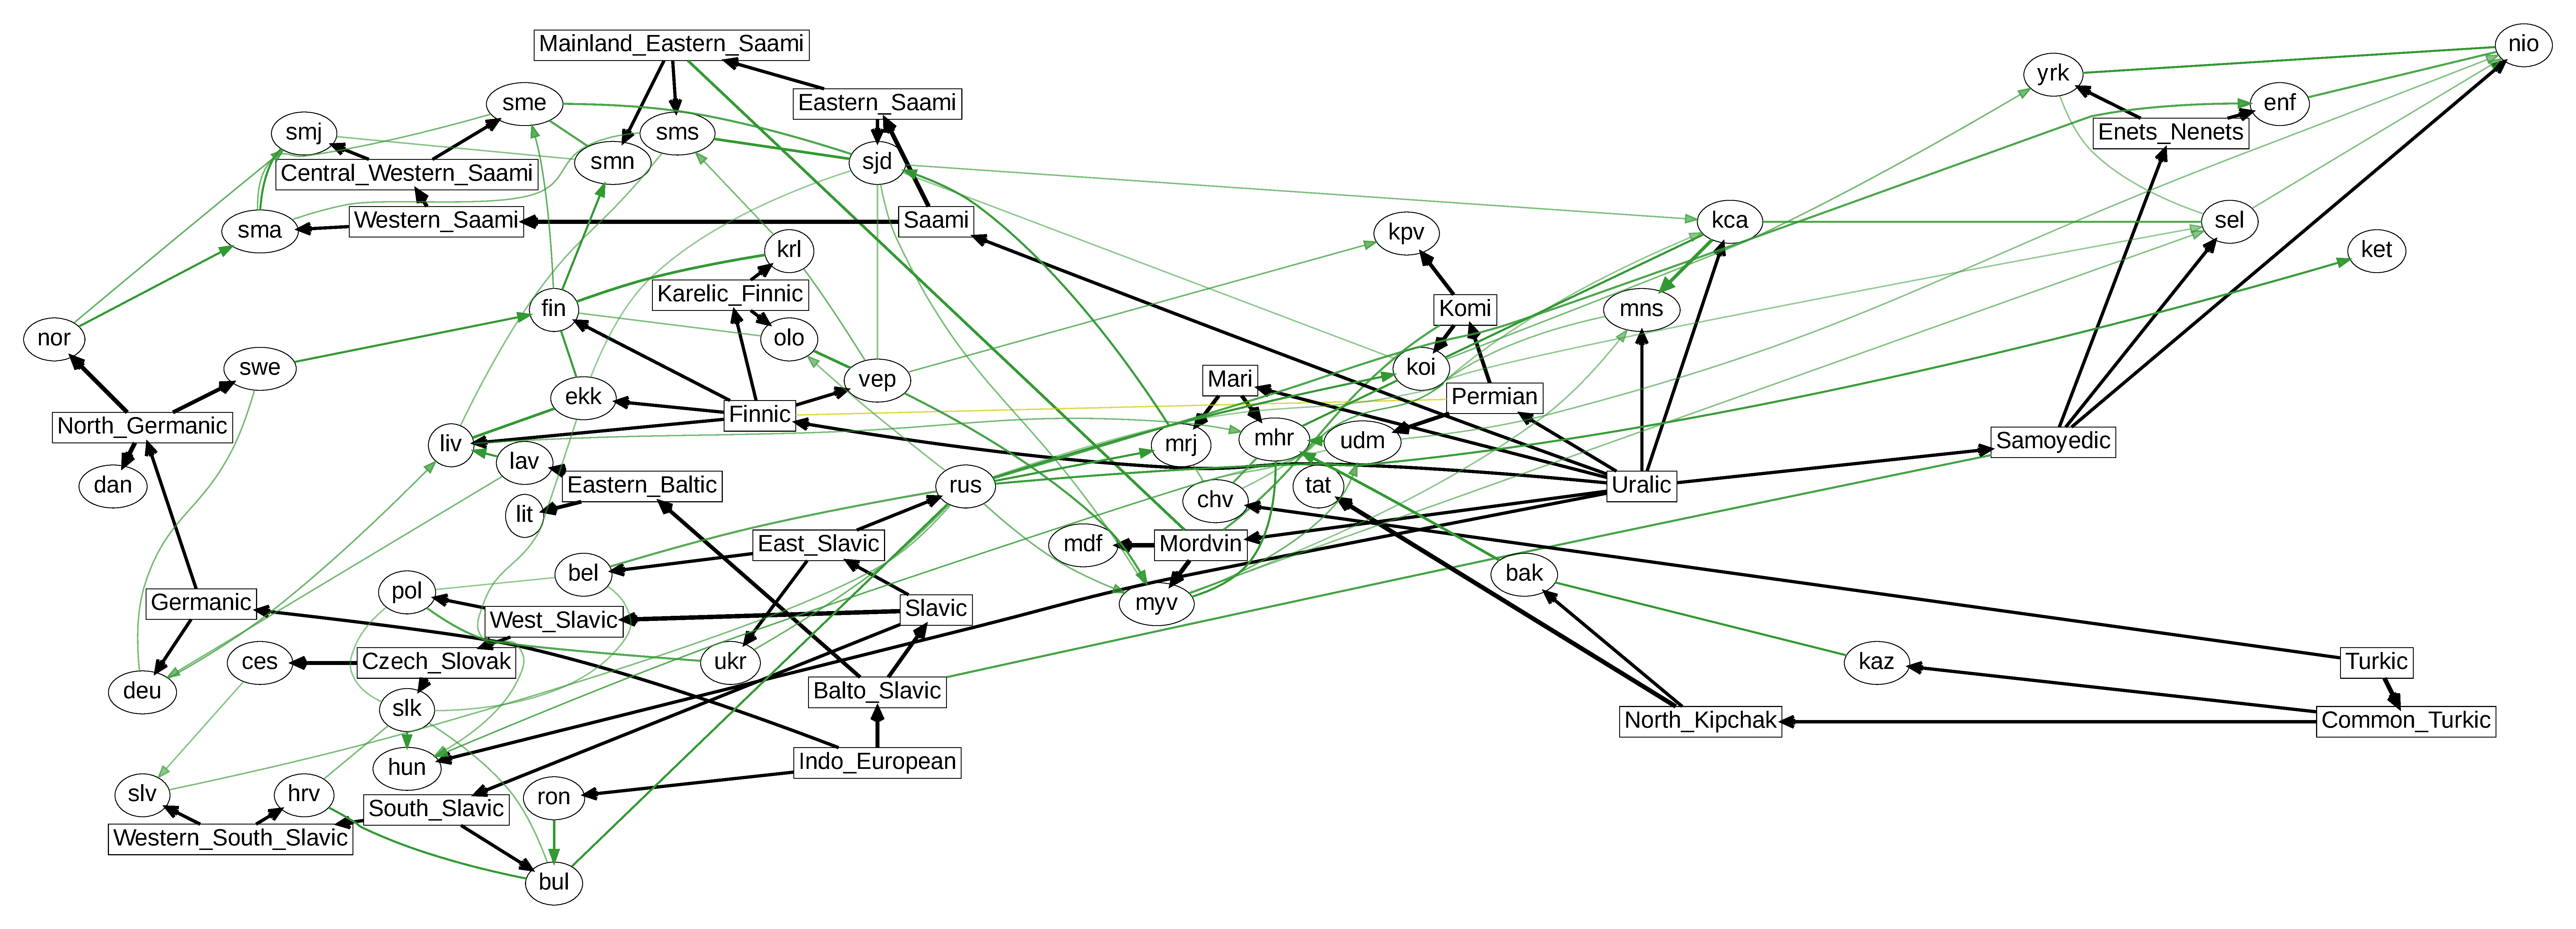
\includegraphics[width=\textwidth]{figures/uralic-fs-ufr-ml-multi.pdf}
 \vspace*{5mm}
 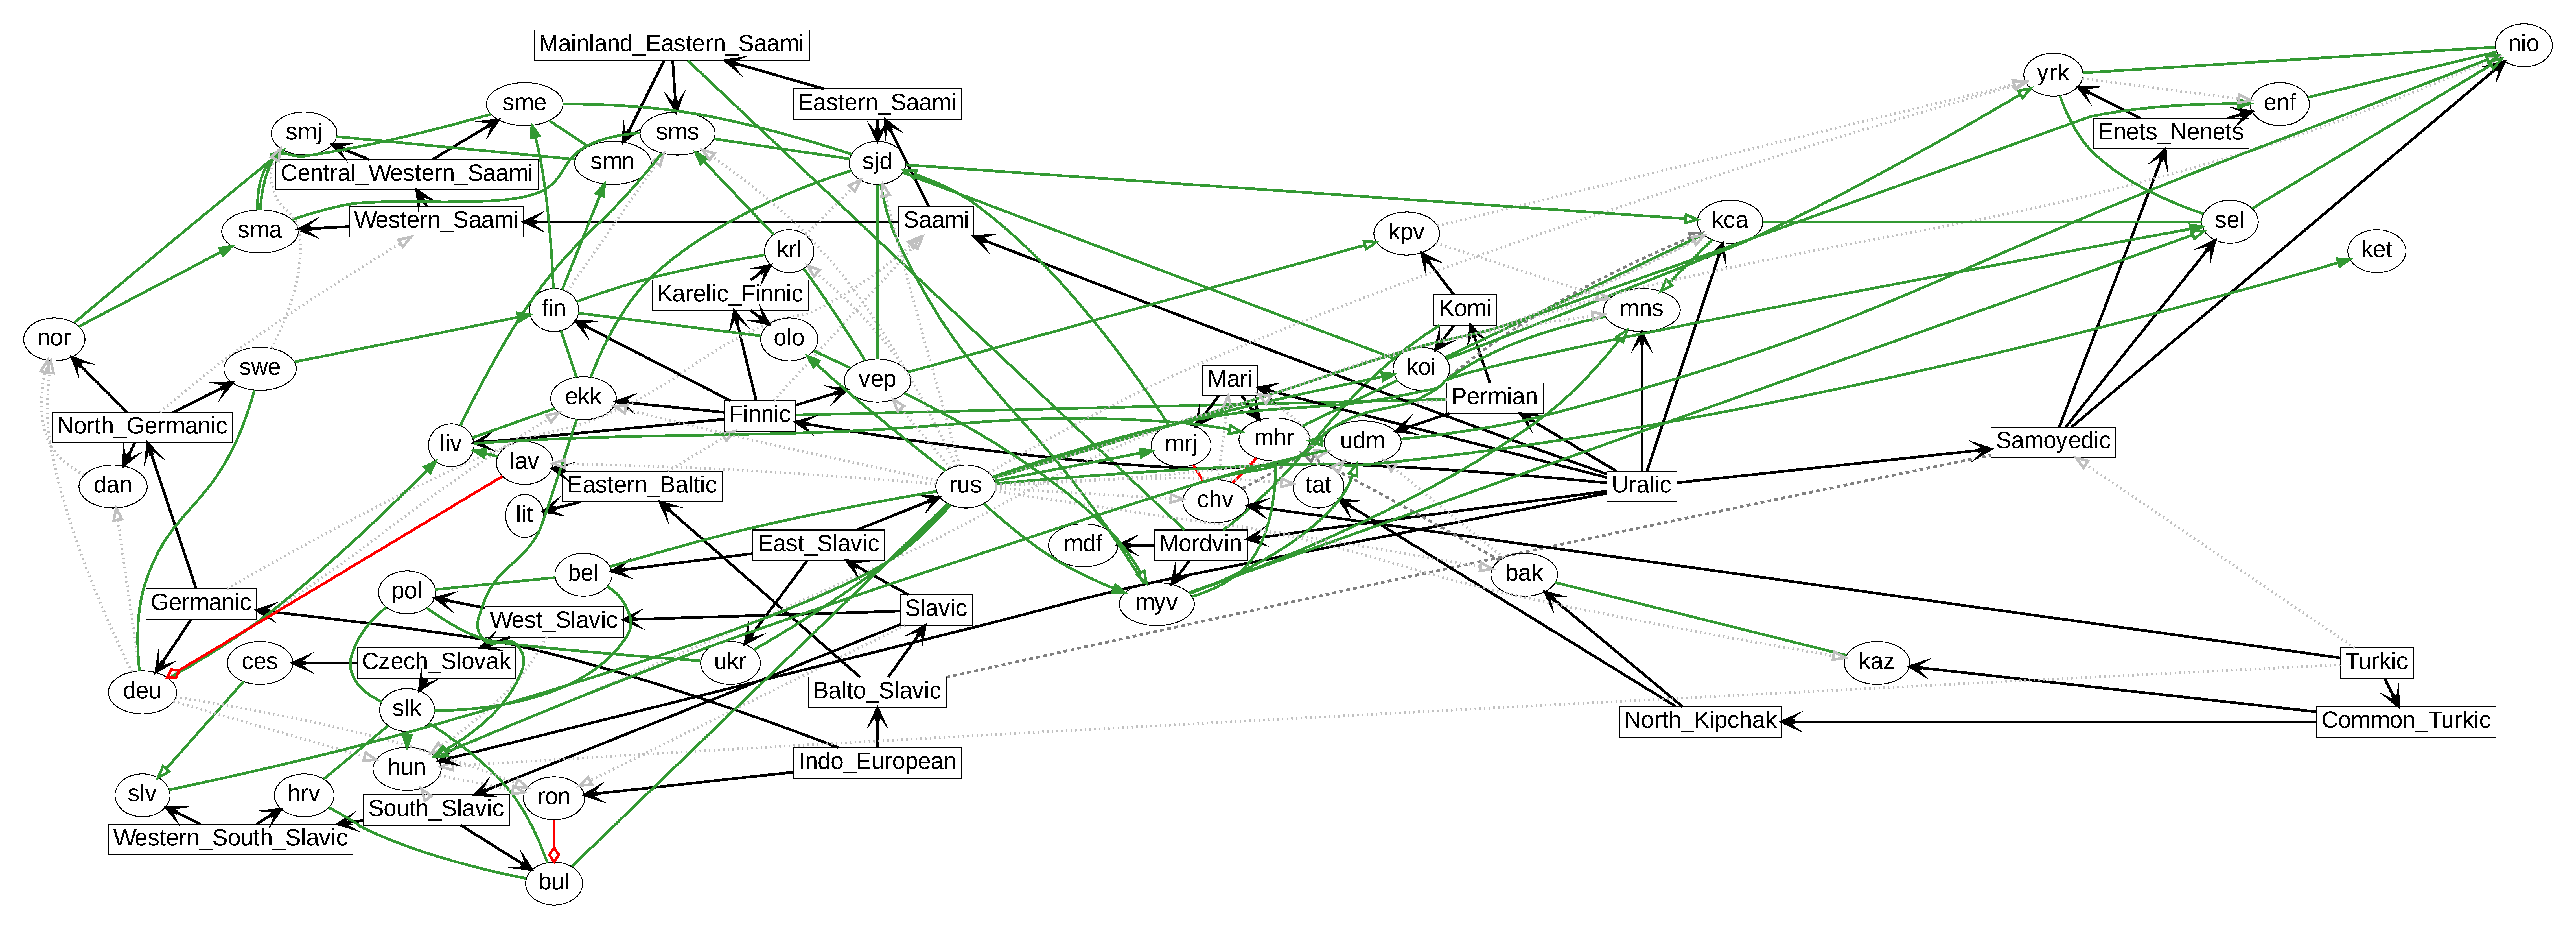
\includegraphics[width=\textwidth]{figures/uralic-fs-ufr-ml-multi-eval.pdf}
 \caption{Result and evaluation of phylogenetic flow on Uralic data}
 \label{uralic-result-phylo}
 \end{sidewaysfigure}
 
 \subsubsection{Case study 3: the linguistic landscape of Siberia}
 The Siberian data display the same large-scale pattern which we already saw in European Russia: all the minority languages have borrowed much of the vocabulary for modern life from \ili{Russian}. As desired, this pattern also appears as the dominant feature of the linguistic area in the inferred lexical flow network visualized in \figref{siberia-result-phylo}. However, two of the arrows, the ones from Russian to \ili{Sakha} (\iso{sah}) and \ili{Evenki} (\iso{evn}), do not have the desired direction. Again, the reason lies in incorrect results of v-structure tests. The triangle \iso{bua} $\arrowLL$ \iso{sah} $\arrowLL$ \iso{rus} does not look at all like a v-structure, because a very large part of the material shared between Russian and \ili{Buryat} (\iso{bua}) is also shared with Sakha, to the point where in a similar pattern to the German-Livonian problem discussed before, conditioning on Sakha actually screens off Russian from Buryat. Due to the failed v-structure test, the correct arrow from Buryat into Sakha is propagated into Russian. The other failed test is for the v-structure \proto{Tungusic} $\arrowLA$ \iso{evn} $\arrowAL$ \iso{rus} which again misses the UFR criterion, albeit at a rather low UFR score of 0.057. Since the inheritance from Tungusic\il{Tungusic languages} is fixed, the only way to resolve this triple in such a way that no v-structure arises, is again by inferring an arrow into Russian.
 
 Coming to the spurious connections, the influence of \ili{Russian} on the two \ili{Yukaghir languages} was detected as going into Pro\-to-Yu\-ka\-ghir, again because of the impossibility for the reconstruction algorithm to decide that a cognate class appearing in both daughter languages should not be projected to the proto-lan\-guage. Assuming two separate arrows into the two individual languages is simply not the parsimonious solution if we do not include the knowledge that Proto-Yukaghir had already ceased to exist when the Yukaghirs were colonized. Exactly the same problem also leads to the spurious connections between Russian and Proto-Chukotko-Kamchatkan\il{Chukotko-Kamchatkan languages} as well as between Russian and Eskimo-Aleut\il{Eskimo-Aleut languages}.
 
 An erroneous v-structure \iso{sah} $\arrowAA$ \iso{xal} $\arrowAL$ \iso{kaz} is inferred due to zero unique flow between the \ili{Turkic languages} across the Mongolic language \iso{xal}\il{Kalmyk}, indicating that the true pattern \iso{sah} $\arrowAL$ \iso{xal} $\arrowAL$ \iso{kaz} is very unlikely. In fact, the inferred configuration is not as incorrect as the evaluation criteria imply. Arrows between \iso{xal} and \iso{kaz}\il{Kazakh} in both directions can be justified based on the gold standard, as it includes arrows \proto{Mongolic} $\arrowLA$ \iso{kaz} and \proto{Kipchak} $\arrowLA$ \iso{xal}. The problem can thus be reduced to the fact that \proto{Kipchak} is not a node in the reduced tree for this scenario, because other Kipchak languages\il{Kipchak Turkic languages} like \ili{Bashkir} and \ili{Tatar} are not part of the language sample.
 
 The spurious connections of \ili{Selkup} (\iso{sel}) to \ili{Chinese} and \ili{Itelmen} are due to a slightly too high noise level in cognate detection. For instance, Selkup and Chinese have an overlap of 28 cognate classes according to the inferred cognacy relation, and the 0.025 threshold would have kicked in at 25 cognate classes. This scenario also provides a nice example for why spurious connections are very problematic, because the Selkup-Chinese connection is also responsible for the inverted arrow from \ili{Japanese} into Chinese, due to an inferred v-structure \iso{sel} $\arrowLA$ \iso{cmn} $\arrowAL$ \iso{jpn}. Still, by focusing only on all of these problems one must not forget that in many other cases, PLFI works just as intended, and that many of these errors will disappear under the TSS directionality criterion, again making the case for a combined approach to enhance stability.
 
\begin{sidewaysfigure}
 
\includegraphics[width=0.8\textwidth]{figures/siberia-fs-ufr-ml-multi.pdf}
 \vspace*{5mm}
 
\includegraphics[width=0.8\textwidth]{figures/siberia-fs-ufr-ml-multi-eval.pdf}
 \caption{Result and evaluation of phylogenetic flow on Siberian data}
 \label{siberia-result-phylo}
\end{sidewaysfigure}

\subsubsection{Case study 4: a visit to the Caucasus}
With the Caucasus scenario, we finally encounter the most complex test case. As can be seen on visual inspection of the evaluation graph in \figref{caucasus-result-phylo}, the more peripheral influences from \ili{Arabic} and \ili{Russian} into the Caucasus area are inferred correctly, but in the chaotic situation among Caucasian languages, there is just too much interacting and contradictory signal for PLFI to perform well.
 
The problems within Daghestanian\il{Daghestanian languages} might also be due to imperfections in the gold standard (the Caucasus being the only region where it was almost impossible to find literature on language contacts for some languages), but the case of \ili{Georgian} (\iso{kat}), an isolate in this dataset, points to a further issue that requires some consideration.
 
The underlying signal indicating language contact always comes in the shape of cognate classes present in some child language of an ancestral language which does not contain them, but a more distant language does. This is the pattern which makes the data non-tree-like, and causes lateral connections that cannot be explained away. Now, the directionality inference can recognize that the recipient language is a mixture of its own ancestor and the donor language. This entire mechanism cannot work reliably for isolated languages, because there is no proto-language in the model, and if we assumed an additional proto-language representing an earlier stage of the isolate, the reconstruction algorithm could not decide based on the single descendant language which cognate classes must have existed at that node, and would project all the inherited material up into the proto-language. The only reason why the arrow from Russian into the Siberian isolate Ket was inferred successfully in the previous case study was the other erroneous arrow from Sakha into Russian. This problem only occurs among isolates, however. An additional Slavic language in the dataset would have shared most of the Russian loans as well, and Proto-Slavic would have provided the necessary third language for a negative collider test involving the link from Ket into Russian. In a sense, the method faces the same limitations which historical linguists face when trying to infer the directionality of loans between isolates. This is notoriously difficult to do, and can only be done when loanwords are recognizable due to language-internal reasons, e.g.\ because they do not adhere to some phonological constraints governing the rest of the lexicon.
 
Finally, let us investigate  why the important connections \iso{tur} $\arrowLA$ \iso{kmr} and \iso{pes} $\arrowLA$ \iso{tur} could not become part of the skeleton. The reason is that with \ili{Azeri} (\iso{azj}), there is another Turkic language that is lexically very close to \ili{Turkish}, but has interacted with both \ili{Iranian languages} even more, because of lexical contact on a more equal footing with \ili{Kurdish} as minority languages of Iran. The overlap of Azeri with \ili{Persian} and Kurdish therefore subsumes the overlaps of both languages with Kurdish, leaving only the links with Azeri in the skeleton. The signal behind the spurious arrow from Azeri into Kurdish is actually the one which should have created the missing arrow from Turkish into Kurdish.
 
Finally, let us explore why the nature of \ili{Azeri} and \ili{Uzbek} as \ili{Turkic languages} with many \ili{Persian} loans is not understood by the algorithm, which instead produces the wrongly directed arrows \iso{azj} $\arrowLA$ \iso{pes} and \iso{uzn} $\arrowLA$ \iso{pes}. Here, Persian is the language which looks like a mixture of elements of Azeri and Uzbek, the assumed transmitted material being exactly the Persian loans the two Turkic languages share, because these are projected into and then explained by Turkic. On a more abstract level, this phenomenon is another example of how the indistinguishability of inherited words and widespread loans can result in erroneous arrows. Unlike other erronous v-structures, this is purely a reconstruction problem which also hits the TSS criterion, where the arrow \iso{uzn} $\arrowLA$ \iso{pes} has an evidence ratio of $3.575$. In the global NorthEuraLex network, this problem does not occur, because the many other Turkic languages untouched by Persian produce a Turkic reconstruction that does not 
contain any of these. The situation could therefore be improved by considering more Turkic languages. It is an interesting question whether to a historical linguist, all the Persian elements in Turkish and Uzbek would actually be recognizably foreign if only three Turkic languages were attested.
 
  \begin{figure}[ht!]
 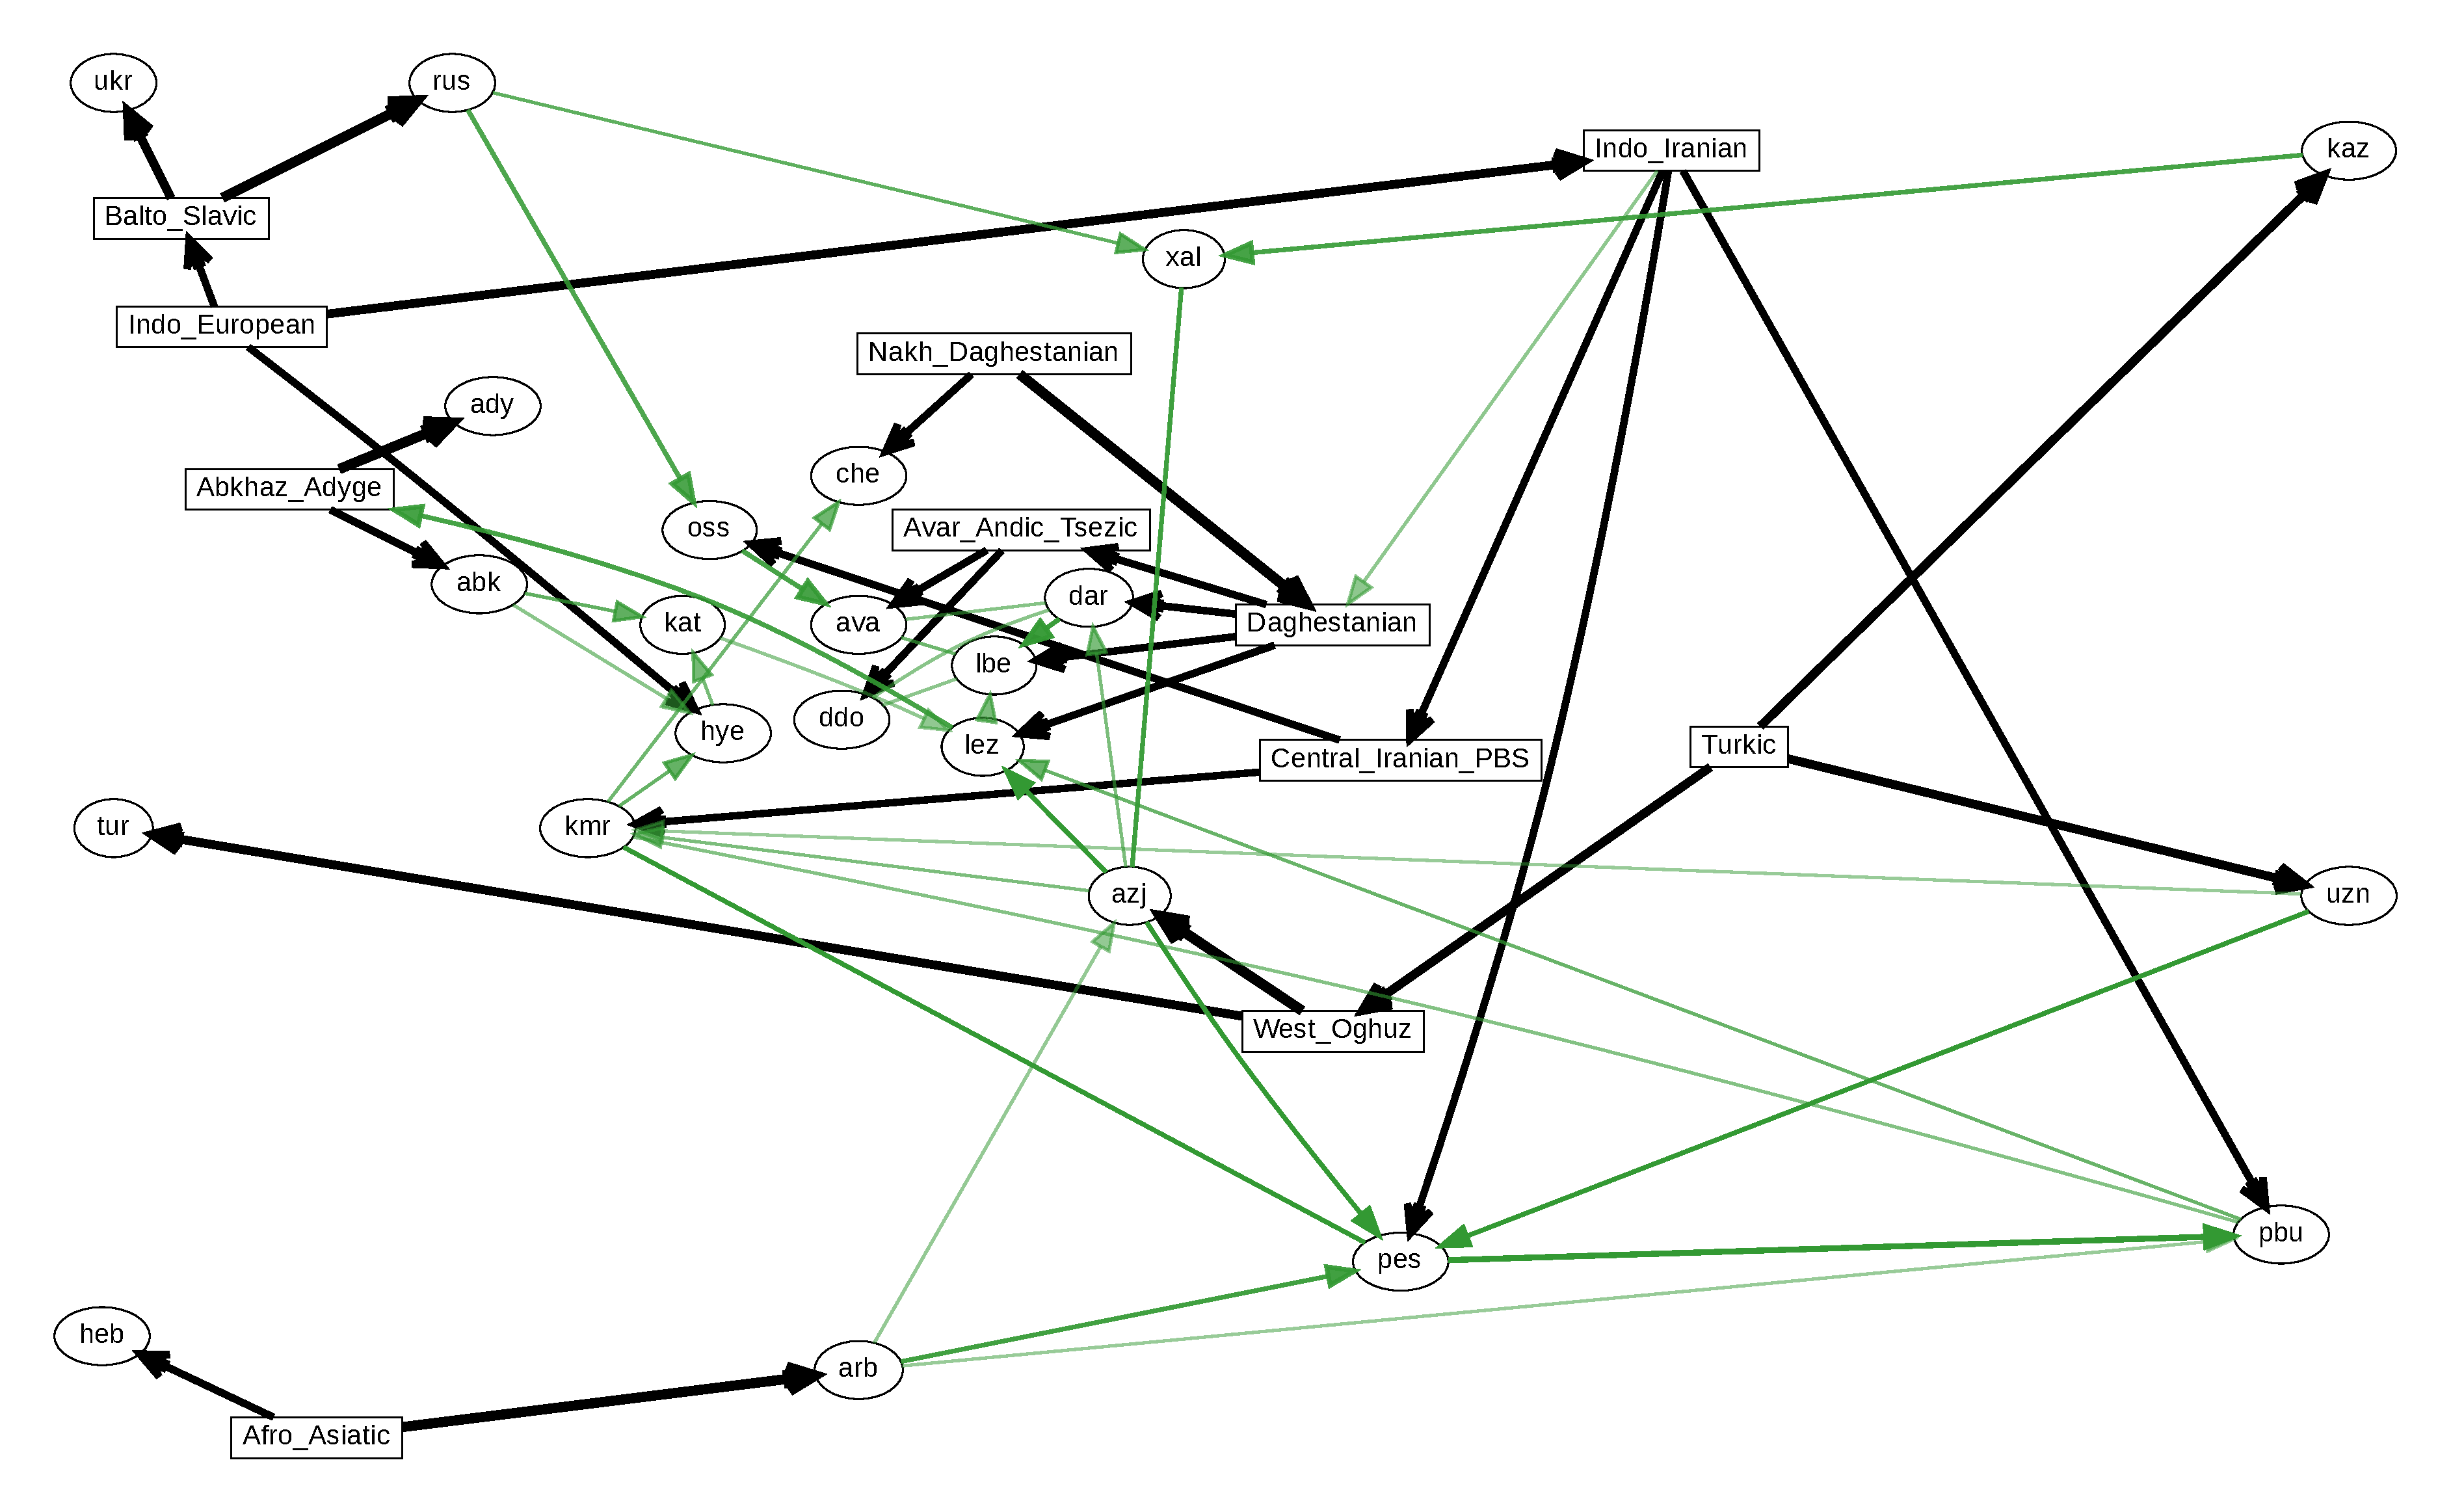
\includegraphics[width=\textwidth]{figures/caucasus-fs-ufr-ml-multi.pdf}
 \vspace*{5mm}
 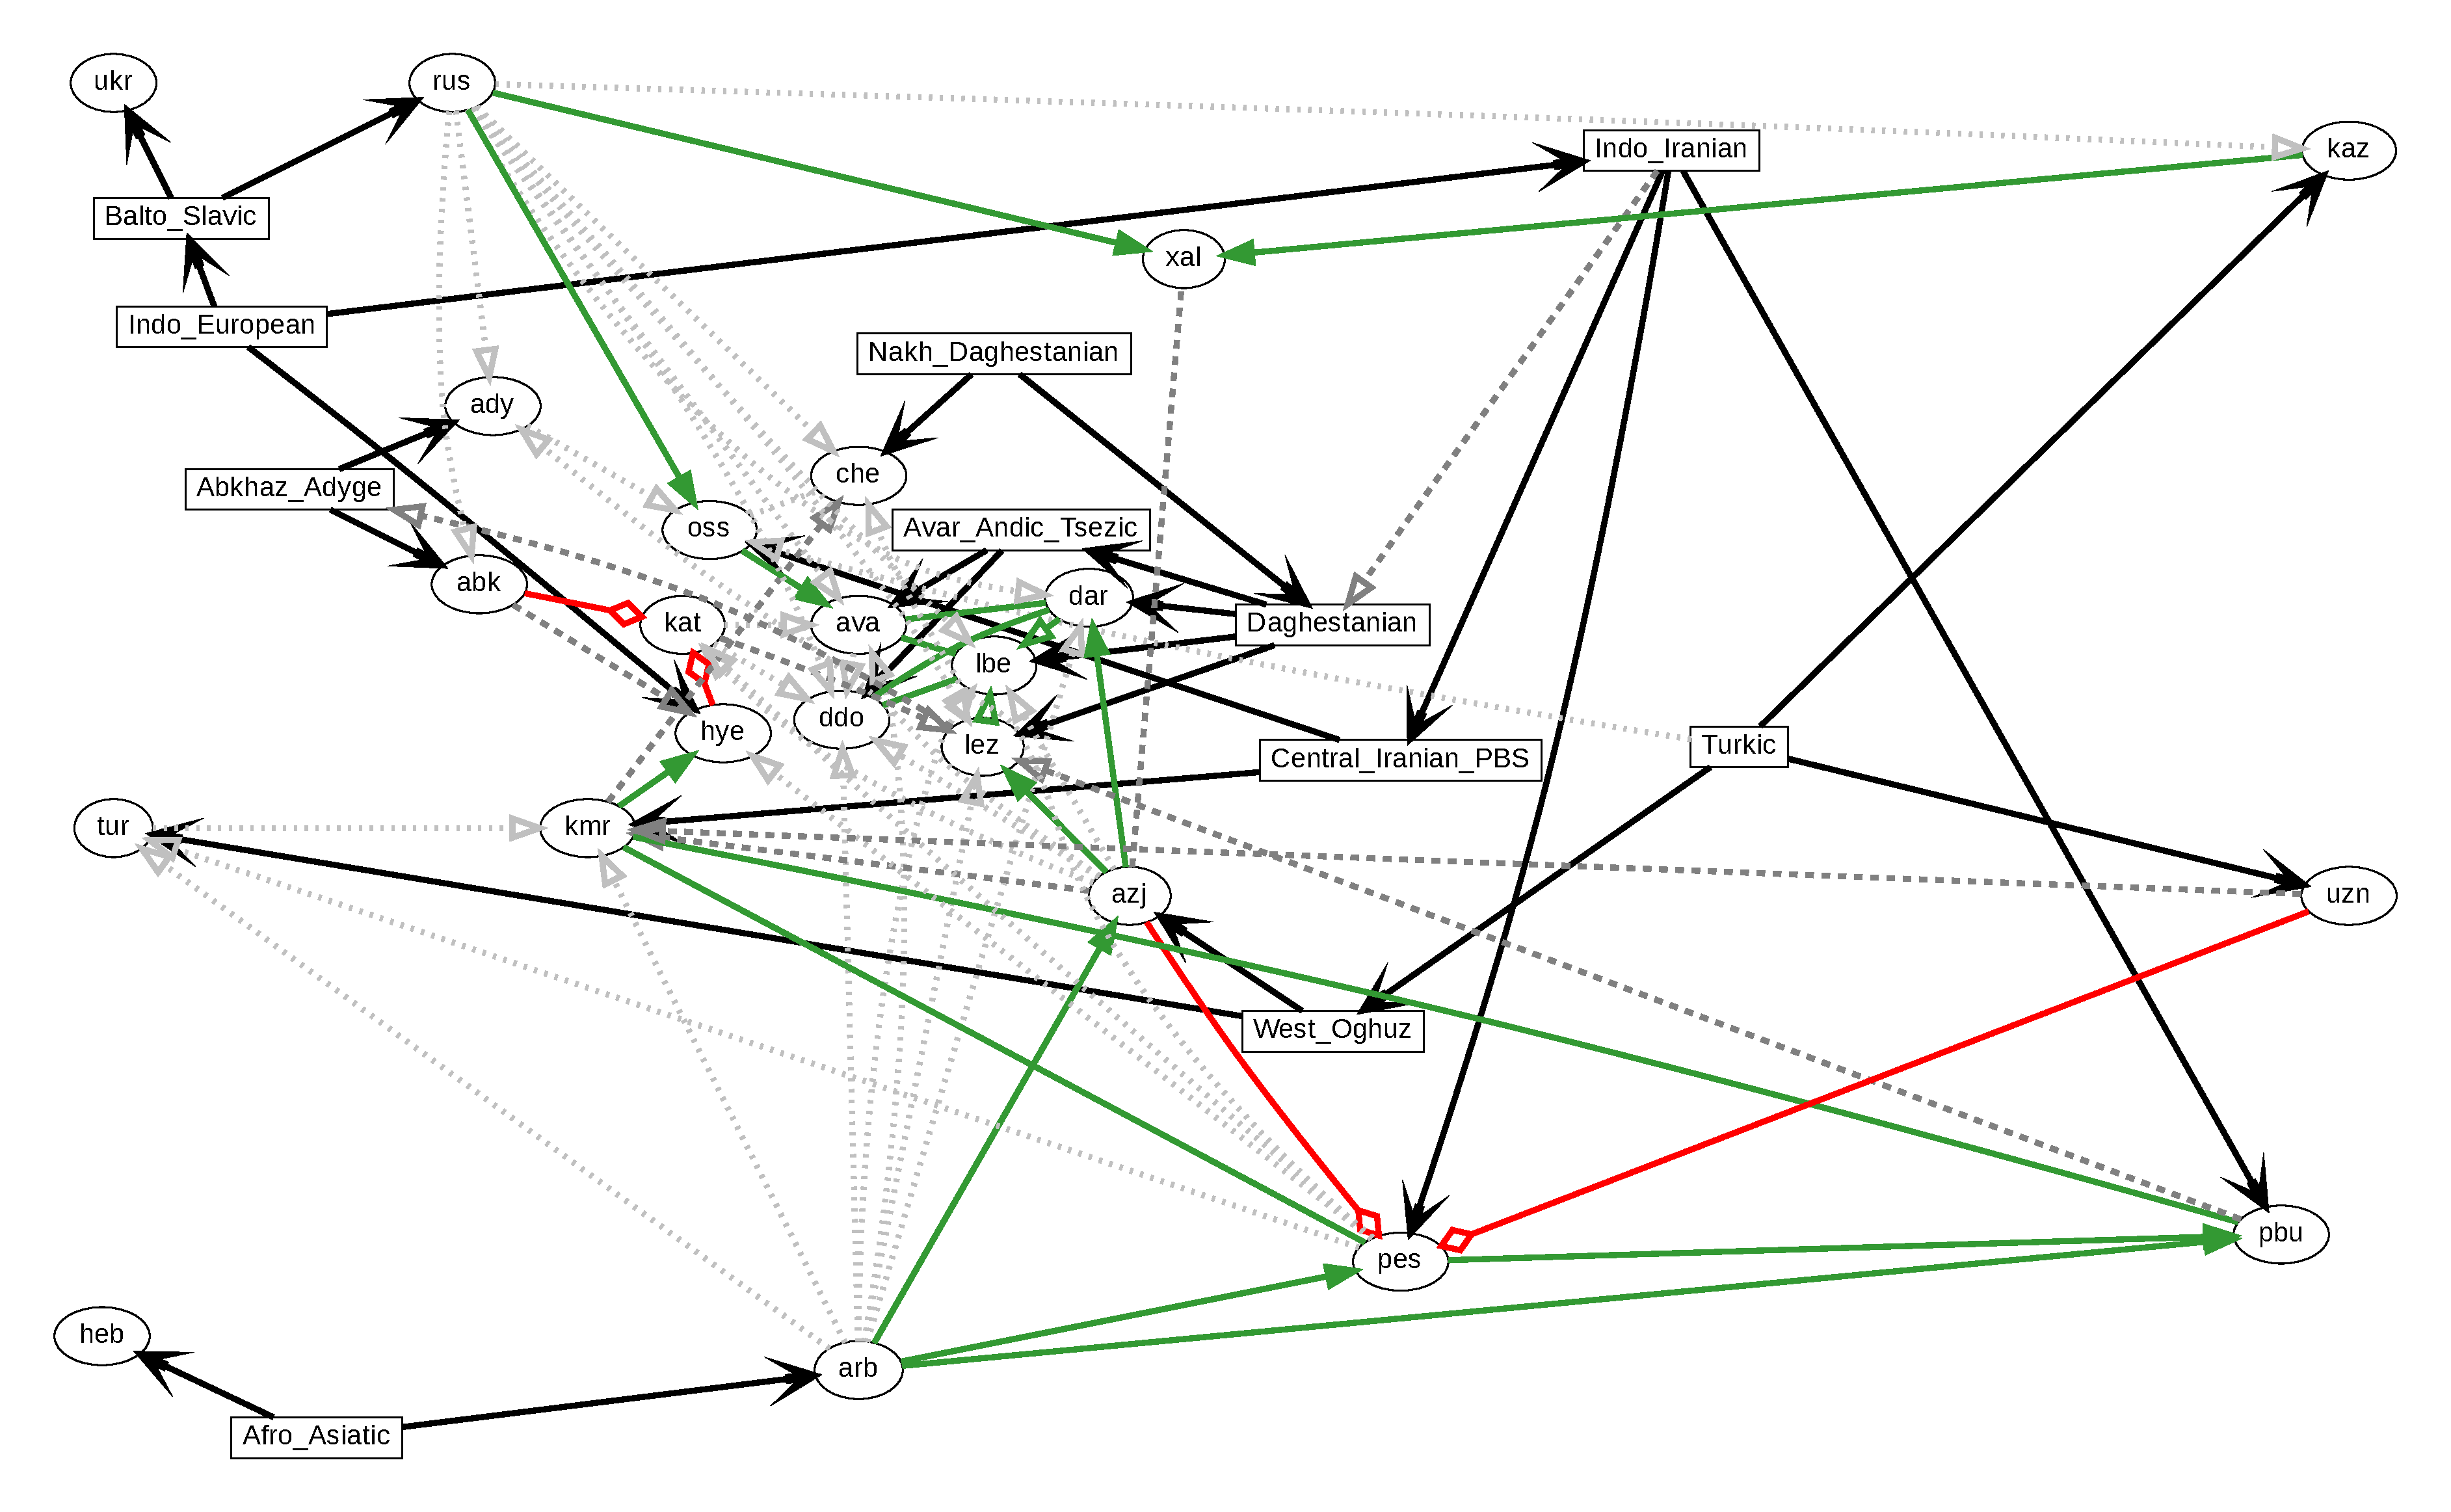
\includegraphics[width=\textwidth]{figures/caucasus-fs-ufr-ml-multi-eval.pdf}
 \caption{Result and evaluation of phylogenetic flow on Caucasian data}
 \label{caucasus-result-phylo}
 \end{figure}

\subsection{Evaluation on simulated data}
As the final analysis in this chapter, we now return to the simulated data. There are two important questions answers to which the simulated data will help us find. First, we want to quantify how much potential performance we lost by using ancestral state reconstruction methods and acting as if the reconstructed data were actually observed. Second, we want to know whether the performance on the simulated data is comparable to what we observed on NorthEuraLex, and whether our previous findings about the relative advantages of the different skeleton and directionality inference methods generalize beyond my dataset.

We start by comparing the skeleton performance measures for the three skeleton inference methods on the perfect data (i.e.\ the picture we get if we take the actual states of the simulation when the proto-languages split) to the results on the two best reconstructions. The results are given in \tabref{perfect-vs-reconstruction-skeleton}. If the best skeleton inference method is picked on both types of data, we see an only moderate decrease in F-score from about 87\% to 79\% for the more exact single-value reconstruction, and to 74\% for the more generous multi-value reconstruction. Precision and recall suffer about equally, showing that the reconstructed data contain a more noisy version of the same signal. We see that a good reconstruction method can help us a long way towards results comparable to what we would get on perfect data, confirming our impression that it is possible in principle to extract information about historical language contacts from a cognacy-encoded dataset covering only their living descendants. Interestingly, while flow-separation methods worked best for the NorthEuraLex data, the performance of PS is comparable on perfect data, and even superior on the reconstructed data, especially due to a much higher recall at comparable precision. Interpreting this result, erroneous reconstructions appear to have a rather strong effect on the reliability of connecting paths, indicating that while not clearly superior on perfect data, on noisy reconstructions the PS variant is surprisingly robust.

\begin{table}
 \centering
  \begin{tabular}{cccc}
  \hline \hline
  \# & PrfPC & PrfPS & PrfFS\\ \hline
  skPrc & \textbf{0.901} & 0.870 & 0.829\\
  skRec & 0.780 & \textbf{0.915} & 0.915\\
  skFsc & 0.837 & \textbf{0.892} & 0.870\\
  \hline
 \end{tabular}\\[0.5cm]
 \begin{tabular}{ccccccc}
  \hline \hline
  \# & MLsPC & MLsPS & MLsFS\\ \hline
  skPrc & \textbf{0.851} & 0.798 & 0.711\\
  skRec & 0.539 & \textbf{0.722} & 0.659\\
  skFsc & 0.660 & \textbf{0.758} & 0.684\\
  \hline
 \end{tabular}\\[0.5cm]
\begin{tabular}{ccccccc}
  \hline \hline
  \# & MLsPC & MLsPS & MLsFS\\ \hline
  skPrc & \textbf{0.855} & 0.797 & 0.710\\
  skRec & 0.527 & \textbf{0.720} & 0.658\\
  skFsc & 0.652 & \textbf{0.757} & 0.683\\
  \hline
 \end{tabular}
 \caption{Comparing skeleton performance for perfect ancestral data and the two best reconstructions}
 \label{perfect-vs-reconstruction-skeleton}
\end{table}

The consequences of reconstruction vs. observed data for arrow performance are again not easily quantifiable in our framework, because they result in different skeletons. Still, within each variant we can compare the arrow performance resulting from the different directionality inference methods. To maintain comparability with the NorthEuraLex results, only the numbers for the FS method are given in \tabref{perfect-vs-reconstruction-arrows}. The apparently low arrow performance for the perfect ancestral data is due to the higher skeleton recall, which leaves many weak links in the skeleton where overlaps are small and directionality evidence therefore uncertain.

Instead, these numbers provide us with a further piece of the answer to the second question. Contrary to what we saw on the NorthEuraLex dataset, TSS directionality can now compete with the UFR criterion across reconstructions. The theoretical considerations leading to the TSS method seem to apply much better on this dataset. So what is the underlying reason? The only obvious difference between the two types of scenarios is that the simulated data have perfect cognate clustering, whereas the automated cognate clustering that I performed to derive cognacy overlap data from NorthEuraLex is quite noisy. Essentially, this noise causes non-zero values for $\delta$ even in unshielded colliders, making these more difficult to detect, and preventing the TSS method from reaching its full potential. In contrast, the UFR method can handle noise much better, but as we have seen in the case studies, it tends to run into problems in dense graphs where unshielded triples are rare, which is the case in the Caucasus as well as in many of the simulated scenarios. The fact that the statistical assumptions behind causal inference hold much better for perfect cognacy judgments also shows in the much better performance of the VPC and SPC directionality inference methods on the simulated data. While both were completely useless on noisy cognacy data, on clean cognacy data they do manage to capture some of the signal, although their results remain very unreliable, and the specialized directionality inference methods perform better by a significant margin.

\begin{table}
 \centering
  \begin{tabular}{ccccc}
    \hline \hline
   & \multicolumn{4}{l}{FS on perfect ancestral data}\\ 
   & VPC & SPC & UFR & TSS\\ \hline
  arPrc & 0.414 & 0.362 & \textbf{0.438} & 0.371\\
  arRec & 0.415 & 0.313 & \textbf{0.585} & 0.366\\
  arFsc & 0.414 & 0.336 & \textbf{0.501} & 0.368\\
  \hline
 \end{tabular}\\[0.5cm]
 \begin{tabular}{ccccc}
  \hline \hline
   & \multicolumn{4}{l}{FS on MLsgl reconstruction}\\ 
   & VPC & SPC & UFR & TSS\\ \hline
  arPrc & 0.490 & 0.512 & 0.432 & \textbf{0.555}\\
  arRec & 0.362 & 0.290 & \textbf{0.423} & 0.343\\
  arFsc & 0.417 & 0.370 & \textbf{0.428} & 0.424\\
  \hline
 \end{tabular}\\[0.5cm]
 \begin{tabular}{ccccc}
  \hline \hline
   & \multicolumn{4}{l}{FS on MLmlt reconstruction}\\ 
   & VPC & SPC & UFR & TSS\\ \hline
  arPrc & 0.485 & 0.508 & 0.435 & \textbf{0.561}\\
  arRec & 0.354 & 0.288 & \textbf{0.422} & 0.347\\
  arFsc & 0.409 & 0.368 & 0.428 & \textbf{0.428}\\
  \hline
 \end{tabular}
 \caption{Comparing skeleton performance for perfect ancestral data and the two best reconstructions}
 \label{perfect-vs-reconstruction-arrows}
\end{table}

Again, we can combine skeleton and arrow F-scores by multiplication to derive an overall performance figure for each of the compared methods, which makes it possible to quantify approximately how much overall performance we lose due to reconstruction. The resulting numbers are ranked by the best result on perfect ancestral data in \tabref{variant-comparison-perfect-vs-reconstructed}, which compares the performance on the two reconstructions against the perfect data, also quantifying the losses or gains in percentages. Overall, the FS-UFR variant is clearly the best-performing on the perfect data, whether FS-TSS is the best on reconstructed data. Moreover, most methods perform between 20\% and 30\% worse on both single-value and multi-value ML reconstruction on the perfect data. Encouragingly, the specialized directionality inference method TSS does not follow the general pattern, but provides a method that at less than 10\% decrease is stable against the negative consequences of reconstruction, and this 
at moderate performance.

\begin{table}
 \centering
 \begin{tabular}{cclrlr}
 \hline \hline
PLFI Variant & perfect data & MLsgl & (diff) & MLmlt & (diff)\\ \hline
\texttt{FS-UFR} & 0.436 & 0.293 & (-32.8\%) & 0.293 & (-32.8\%)\\
\texttt{FS-VPC} & 0.360 & 0.285 & (-20.8\%) & 0.279 & (-22.5\%)\\
\texttt{PS-VPC} & 0.346 & 0.273 & (-21.1\%) & 0.271 & (-21.7\%)\\
\texttt{FS-TSS} & 0.320 & 0.290 & (- 9.4\%) & 0.293 & (- 8.4\%)\\
\texttt{PC-VPC} & 0.313 & 0.232 & (-25.9\%) & 0.237 & (-24.3\%)\\
\texttt{FS-SPC} & 0.292 & 0.253 & (-13.4\%) & 0.251 & (-14.0\%)\\
  \hline
 \end{tabular}
 \caption{Analysis of consequences of reconstructed data for selected PLFI variants}
 \label{variant-comparison-perfect-vs-reconstructed}
\end{table}

Finally, we can compare the combined scores to elucidate to what extent the methods behave similarly on the simulated and the NorthEuraLex data. In \tabref{variant-comparison-simulated-and-nelex}, the different variants are ranked by their overall performance on the simulated data, and the equivalent figure on the NorthEuraLex data is given for comparison. The difference in percent, plus the rank of each method in the ranking by performance on the NorthEuraLex data, are given in addition to facilitate interpretation of results. Apart from the already mentioned advantage of TSS on simulated data, and of UFR on noisy-cognate data, the methods agree on four of the top-five methods, and the advantage of specialized skeleton and directionality inference techniques persists for the simulated data. This shows that my findings for NorthEuraLex generalize well to the simulated data, validating both the simulation model and the PLFI paradigm.

\begin{table}
 \centering
 \begin{tabular}{lrrrr}
\hline \hline
PLFI Variant & simulated & NorthEuraLex & difference & rank on NELex\\ \hline
\texttt{MLmlt-FS-UFR} & 0.293 & 0.392 & +0.099 & 1\\  
\texttt{MLmlt-FS-TSS} & 0.293 & 0.349 & +0.056 & 2\\
\texttt{MLsgl-FS-TSS} & 0.293 & 0.344 & +0.051 & 3\\
\texttt{MLsgl-FS-UFR} & 0.290 & 0.324 & +0.034 & 4\\
\texttt{MLsgl-FS-VPC} & 0.285 & 0.081 & -0.204 & 9\\
\texttt{MLmlt-FS-VPC} & 0.279 & 0.110 & -0.169 & 6\\
\texttt{MLsgl-PS-VPC} & 0.273 & 0.098 & -0.175 & 8\\
\texttt{MLmlt-PS-VPC} & 0.271 & 0.134 & -0.137 & 5\\
\texttt{MLsgl-FS-SPC} & 0.253 & 0.043 & -0.210 & 11\\
\texttt{MLmlt-FS-SPC} & 0.251 & 0.000 & -0.251 & 12\\
\texttt{MLmlt-PC-VPC} & 0.237 & 0.098 & -0.139 & 7\\
\texttt{MLsgl-PC-VPC} & 0.232 & 0.045 & -0.187 & 10\\
  \hline
 \end{tabular}
 \caption{Comparison of PLFI variants between datasets}
 \label{variant-comparison-simulated-and-nelex}
\end{table}

To summarize my findings, the PLFI paradigm of reconstructing ancestral cognates and treating them as additional observations in a causal inference paradigm has turned out to work reasonably well, although the quality of results depends a lot on the quality of the reconstruction as well as the choices of skeleton and directionality influence algorithms in the causal framework. The most important positive result of the evaluation is that the recall values for the skeleton are high, indicating that if lateral connections exist in the data, they will generally be present in the lexical flow graph. Also, the skeleton precision values indicate that about three quarters of the lateral connections in the graph will turn out to correspond to actual contacts on closer examination. This shows that PLFI lives up to its promise as a promising exploratory tool for historical linguists in the initial stages of clarifying the linguistic history of a region. Directionality inference is less reliable, but we have seen that in scenarios involving the contacts between larger families (and not isolates), about four out of five inferred arrows will have the correct direction. On the downside, deciding whether influences occurred between extant languages or their ancestors turned out to be very difficult and unstable across different reconstructions, which guides us towards the less ambitious contact flow task that will be tackled in the next chapter.
